\documentclass{patmorin}

\setlength{\parskip}{1ex}

\usepackage{amssymb}
\usepackage{amsmath}
\usepackage{amsthm}
\setcounter{tocdepth}{3}
\usepackage{graphicx}
\usepackage{enumerate}
\usepackage{caption}
\usepackage{subcaption}
\usepackage{subfig} 
%\usepackage[margin=1.2in]{geometry}
\usepackage[usenames,dvipsnames]{xcolor}
\usepackage{tikz}
\usetikzlibrary{shapes,snakes}
\usetikzlibrary{arrows}
\usetikzlibrary{calc}

\let\oldemptyset\emptyset
\let\emptyset\varnothing


\newcommand{\reals}{\mathbb{R}}
\newcommand{\integers}{\mathbb{Z}}
\newcommand{\naturals}{\mathbb{N}}

% \spnewtheorem{claim}{Claim}[lemma]{\itshape}{\itshape}
% \spnewtheorem{claim}{Claim}[theorem]{\itshape}{\itshape}

% \let\lemma\relax % undefine the environment
% \spnewtheorem{lemma}{Lemma}[theorem]{\bfseries}{\rmfamily}
% \spnewtheorem{lemma2}{Lemma}{\bfseries}{\rmfamily}
% \let\lemma\relax
% \spnewtheorem{lemma}[theorem]{Lemma}
%\theoremstyle{definition}
%\newtheorem{definition}[theorem]{Definition}

%For coloured paths
\newcommand{\un}{\textcolour{blue}{1}}
\newcommand{\deux}{\textcolour{green}{2}}
\newcommand{\trois}{\textcolour{brown}{3}}
\newcommand{\quatre}{\textcolour{red}{4}}

%Some useful commands
\newcommand{\block}{\mathrm{block}}
\newcommand{\cycle}{\mathrm{cycle}}
\newcommand{\dist}{{d}}

\newcommand{\wdual}[1]{#1^{\circ}}
\newcommand{\hset}[1]{\mathcal{H}(#1)}

\usepackage{url}
\urldef{\mailsa}\path|{jit,morin,lucasriouxmaldague}@scs.carleton.ca|
\urldef{\mailsb}\path|vida@cs.mcgill.ca|    
\newcommand{\keywords}[1]{\par\addvspace\baselineskip
\noindent\keywordname\enspace\ignorespaces#1}

\newtheorem{theorem}{Theorem}[section]
\newtheorem{lemma}[theorem]{Lemma}
\newtheorem{corollary}[theorem]{Corollary}
\newtheorem{conjecture}[theorem]{Conjecture}
\newtheorem{claim}{Claim}[theorem]
\newtheorem{obs}[theorem]{Observation}


\newcommand{\thmfacialoutplanar}{Let $G$ be an outerplane graph. Then, $\pi_f(G) \leq 11$.}
\newcommand{\thmfacialoutplanarbic}{Let $G$ be an outerplane graph that contains at most one 2-connected component. Then, $\pi_f(G) \leq 7$.}
\newcommand{\thmfacialplanar}{Let $r=\max\{\pi_f(G) \;|\; G \text{ is outerplane}\}$ and let $G$ be a plane graph. Then, $\pi_f(G) \leq 2r$.}

\newcommand*\samethanks[1][\value{footnote}]{\footnotemark[#1]}

% first the title is needed
\title{\MakeUppercase{New Bounds for Facial Nonrepetitive Colourings}}
\date{}

\author{Prosenjit Bose,\thanks{School of Computer Science, Carleton University, Ottawa, Canada. \texttt{jit@scs.carleton.ca}, \texttt{morin@scs.carleton.ca}, \texttt{lucasriouxmaldague@scs.carleton.ca}}\, %
\and Vida Dujmovi{\'c},\thanks{School of Computer Science and Electrical Engineering, University of Ottawa, Ottawa, Canada. \texttt{vida.dujmovic@uottawa.ca}}\,
\and Pat Morin,\samethanks[1]\, \and Lucas Rioux-Maldague\samethanks[1] }

\begin{document}

% \mainmatter  % start of an individual contribution

% a short form should be given in case it is too long for the running head
% \titlerunning{New Bounds for Facial Nonrepetitive Colourings}

% the name(s) of the author(s) follow(s) next
%
% NB: Chinese authors should write their first names(s) in front of
% their surnames. This ensures that the names appear correctly in
% the running heads and the author index.
%
%
%\authorrunning{Bose, Dujmovi{\'c}, Morin \and Rioux-Maldague}
% (feature abused for this document to repeat the title also on left hand pages)

% the affiliations are given next; don't give your e-mail address
% unless you accept that it will be published

% \institute{School of Computer Science, Carleton University,\\
% Ottawa, Canada\\
% \mailsa\\\mailsb\\}

%
% NB: a more complex sample for affiliations and the mapping to the
% corresponding authors can be found in the file "llncs.dem"
% (search for the string "\mainmatter" where a contribution starts).
% "llncs.dem" accompanies the document class "llncs.cls".
%

% \toctitle{Lecture Notes in Computer Science}
% \tocauthor{Authors' Instructions}
\maketitle

\begin{abstract}
A sequence $S=s_1,s_2,\cdots,s_{2r}$ is a \emph{repetition} if
$s_i=s_{r+i}$ for $1 \leq i \leq r$. Let $G$ be a plane graph. A
\emph{facial path} is a path of consecutive vertices on the boundary walk
of a face. A $k$-nonrepetitive facial colouring is a $k$-vertex colouring
such that the sequence of colours of any facial path is nonrepetitive. The
minimum number of colours such that $G$ has a nonrepetitive facial
colouring is denoted by $\pi_f(G)$. We show that $\pi_f(G)\leq 7$ if $G$
is 2-connected outerplane, $\pi_f(G) \leq 11$ if $G$ is outerplane and
$\pi_f(G)\leq 22$ if $G$ is plane. The latter improves the previous best
known bound on nonrepetitive facial colourings of plane graphs by Barat
and Czap (Journal of Graph Theory, 2013).
\end{abstract}


\section{Introduction}
A sequence $S=s_1,s_2,\cdots,s_{2r}$, $r\ge 1$, is a \emph{repetition}
if $s_i=s_{r+i}$ for $1 \leq i \leq r$. For example, 1212 is a
repetition, while 1213 is not. Repetitions are also referred to as
``squares'', since they can be written as $aa=a^2$. A \emph{block}
of a sequence $S$ is any subsequence of consecutive terms in $S$. A
sequence is \emph{nonrepetitive} (square free) if for every block $B$
of $S$, $B$ is not a repetition. Otherwise $S$ is \emph{repetitive}. For
example, 1312124 is repetitive, as it contains the block 1212 which is a
repetition, while 123213 is nonrepetitive as it contains no such block.
It is easy to see that no sequence of length greater than 3 on two symbols
can be nonrepetitive. A result by Axel Thue in 1906 states
that nonrepetitive sequences of arbitrary length can be created using
three symbols \cite{thue1906uber}. A variant of this problem concerning
graphs was proposed by Alon, Grytczuk, Ha{\l}uszczak and Riordan in
2002 \cite{alon2002nonrepetitive}. This problem has received much
attention since \cite{barat2013facial, barat2007square, barat2008note,
brevsar2007nonrepetitive, currie2002cycle18, dujmovic2012planarlogn,
dujmovic2011nonrepetitive, fiorenzi2011thue, gonccalves2014entropy,
grytczuk2007nonrepetitivesurvey, grytczuk2007nonrepetitive,
grytczuk2013new, harant2012nonrepetitive, kozik2013nonrepetitive,
kundgen2008nonrepetitive, pezarski2009non, schreyer2012facial,
schreyer2013total}. 

A \emph{vertex colouring} or a \emph{proper vertex colouring} of a graph $G$ is a function $c: V(G) \rightarrow \naturals$ that satisfies:
\begin{equation}
c(u) = c(v) \Rightarrow \{u,v\} \notin E(G).
\label{eqn:propervcolouring}
\end{equation}
for all $u,v \in V(G)$. For $k \in \naturals$, a \emph{vertex $k$-colouring} is a proper vertex colouring $c : V(G) \rightarrow \{1,\cdots,k\}$.
A \emph{nonrepetitive vertex $k$-colouring} of a graph $G$ is a vertex $k$-colouring $c$ in which for every vertex path $(v_1,\cdots,v_n)$ in $G$, the sequence $c(v_1),\cdots, c(v_n)$ is nonrepetitive. The \emph{Thue chromatic number} of a graph $G$, denoted $\pi(G)$, is the least $k$ for which a nonrepetitive vertex $k$-colouring of $G$ exists. Some upper bounds on $\pi$ are known: a result by Alon et al.~\cite{alon2002nonrepetitive} (later tightened by Dujmovi\'c et al. \cite{dujmovic2011nonrepetitive}), states that $\pi(G) \in O(\Delta(G)^2)$ where $\Delta(G)$ is the maximum degree of $G$, and this result is tight up to a logarithmic factor.  A famous conjecture relates to the Thue chromatic number of planar graphs:
\begin{conjecture}[Alon et al. \cite{alon2002nonrepetitive}]
 There is a constant $K$ such that $\pi(G) \leq K$ for any planar graph $G$.
 \label{conj:planarConstant}
\end{conjecture}
This conjecture remains open. The current best bound for planar graphs depends on the number, $n$, of vertices and states that $\pi(G) \leq 8(1+\log_{3/2}n)$ \cite{dujmovic2012planarlogn}. We do not know how tight that bound is, but current evidence suggests that it is not tight, as no planar graph with Thue chromatic number greater than 11 is known \cite{dujmovic2012planarlogn}. 

When restricted to some families of planar graphs, Conjecture~\ref{conj:planarConstant} is known to be true.  K{\"u}ndgen and Pelsmajer \cite{kundgen2008nonrepetitive} showed that $K=12$ for outerplanar graphs and $K=4^t$ for graphs of bounded treewidth $t$. The latter bound is tight if $t=1$ (trees), but it is not known if it is tight for other values of $t$. Even the upper bound of 12 for outerplanar graphs is not known to be tight, as no outerplanar graph with Thue number greater than 7 is known \cite{barat2007square}.

In this paper, we consider a variation of Thue colourings
for plane graphs in which we only require facial paths to be
nonrepetitive.
A \emph{plane graph} $G$ is a fixed embedding of a graph in the plane such that its edges intersect only at their endpoints. An \emph{outerplane} graph $G$ is a plane graph such that all the vertices of $G$ are adjacent to the outside face of $G$. 
A \emph{closed walk} in a graph $G$ is a sequence of vertices $v_0,\ldots,v_{\ell-1}$ such that, for every $i\in\{0,\ldots,\ell-1\}$ the edge $v_iv_{(i+1)\bmod \ell}$ is in $E(G)$.
A \emph{facial walk} in a plane graph $G$ is a closed walk
$v_0,\ldots,v_{\ell-1}$ such that, for every $i\in\{0,\ldots,\ell-1\}$,
the edges $v_{(i-1)\bmod \ell} v_i$ and $v_iv_{(i+1)\bmod\ell}$ occur
consecutively in the counterclockwise cyclic ordering of the edges
incident to $v_i$ in the embedding of $G$.
A \emph{facial path} is a contiguous subsequence of a facial walk that
is a path in $G$. 

An edge-colouring variant of facial non-repetitive colouring was first introduced
by Havet et al. \cite{havet2011facial}, then Harant and Jendrol
\cite{harant2012nonrepetitive} followed up with results for the
vertex-colouring setting we study here. A 
\emph{nonrepetitive facial $k$-colouring} is a vertex
$k$-colouring in which for every facial path $(v_1,\cdots,v_n)$ in $G$,
the sequence $c(v_1),\cdots, c(v_n)$ is nonrepetitive. The \emph{facial
Thue chromatic number} of a graph $G$, denoted $\pi_f(G)$, is the least
$k$ for which a nonrepetitive facial $k$-colouring of $G$ exists. As with
Conjecture \ref{conj:planarConstant} for the Thue chromatic number, it
was also conjectured by Harant and Jendrol \cite{harant2012nonrepetitive}
that there exists a constant $K$ such that $\pi_f(G) \leq K$ for any plane
graph $G$. This conjecture was confirmed with $K=24$ by Barat and Czap
\cite{barat2013facial}, and with smaller values of $K$ when restricted
to some families of 2-connected\footnote{A graph is $k$-connected if
it contains more than $k$ vertices and has no vertex cut of size less
than $k$.} plane graphs such as Halin graphs ($K=??$) and Hamiltonian plane
graphs ($K=16$) \cite{harant2012nonrepetitive}. Any nonrepetitive colouring is
also a facial nonrepetitive colouring so we have that $\pi_f(G) \leq
\pi(G)$. The best lower bound for the facial Thue chromatic number is
5 for plane graphs and 4 for outerplane graphs \cite{barat2013facial}.

TODO: Ask Lucas where Halin graphs come from?

In the next sections, we prove tighter bounds for the facial Thue chromatic number of outerplane and plane graphs. Our technique consists in finding a \emph{blocking set}, from which we construct a \emph{blocking graph}. The blocking set is such that its removal from the outerplane graph results in a forest, for which a nonrepetitive 4-colouring exists. We show that a facial nonrepetitive colouring of any outerplane graph can be obtained by combining this colouring of a forest and a facial nonrepetitive colouring of the blocking graph.
We then proceed to show how to find a nonrepetitive colouring on at most 7 colours of the blocking graph. Although it seems hard --- if not impossible --- to find a such a colouring if the blocking graph contains odd cycles, we show that this is feasible if all cycles are even, and that it is possible to select the blocking set as such.

From this technique, we show that the facial Thue chromatic number of a plane graph is bounded by 22, by 11 for outerplane graphs and by 7 for 2-connected outerplane graphs. Let $G$ be a graph and $H$ be a subgraph of $G$. $G[H]$ is the subgraph of $G$ induced by $V(H)$. Let $G$ be a plane graph. $\wdual{G}$ is the \emph{weak dual} of $G$, the subgraph of the dual of $G$ whose vertices correspond to the bounded faces of the $G$. A $k$-connected component of $G$ is a maximal induced subgraph $H$ of $G$ that is $k$-connected.


\section{Preliminary Results}

Before proceeding with our results, we will introduce a helper lemma and two major results which will be used throughout the paper. The lemma is due to Havet et al. \cite{havet2011facial} and provides a way to interlace nonrepetitive sequences.

\begin{lemma}
\label{lem:nonrep_alternate}
 Let $A=A_1,A_2,\ldots,A_k$ be a nonrepetitive sequence over an alphabet $\mathcal{A}$ in which each $A_i$ has size at least 1. For each $i \in \{0,\ldots,k\}$, let $B_i$ be a (possibly empty) nonrepetitive sequence over an alphabet $\mathcal{B}$. If $\mathcal{A} \cap \mathcal{B} = \emptyset$, then
 $ S = B_0, A_1, B_1, \ldots, A_k, B_k$ is a nonrepetitive sequence.
\end{lemma}

We will require two results about the Thue chromatic number of trees and cycles:

\begin{theorem}[Alon et al. \cite{alon2002nonrepetitive}]
 Let $T$ be a tree. $\pi(T) \leq 4$.
 \label{thm:four_colouring_trees}
\end{theorem}

\begin{theorem}[Currie \cite{currie2002cycle18}]
 Let $C_n$ be a cycle on $n > 2$ vertices. 
 $$
 \pi(C_n) = \begin{cases}
             4 & \text{ if } n \in \{5,7,9,10,14,17\} \\
             3 & \text{ otherwise. }
            \end{cases}$$
 \label{thm:colouring_cycles}
\end{theorem}

\section{Outerplane Graphs}

We are now ready to present our results concerning the facial Thue chromatic number of outerplane graphs.
In order to do this, we will first study \emph{blocking sets} of outerplane graphs. Blocking sets play a crucial role in isolating subsets of vertices from each other in a graph. This splits the graph in various parts which are easier to colour, and the specific properties of the blocking set makes it possible to reassemble the graph together without creating repetitions. 

\subsection{Blocking Sets}

Let $G$ be an outerplane graph. A \emph{blocking set} of $G$ is a set
of vertices $B \subseteq V(G)$ such that for each 2-connected component
$H$ of $G$, $H \setminus B$ is a tree and for each inner face $F$,
$F \setminus B \not= \emptyset$. 
Observe that $G\setminus B$ is a forest that contains a non-empty tree
for each 2-connected component of $G$.
See Figure \ref{fig:blocking_set} for an example of a blocking set. 

\begin{figure}[!ht]
  \centering
  
  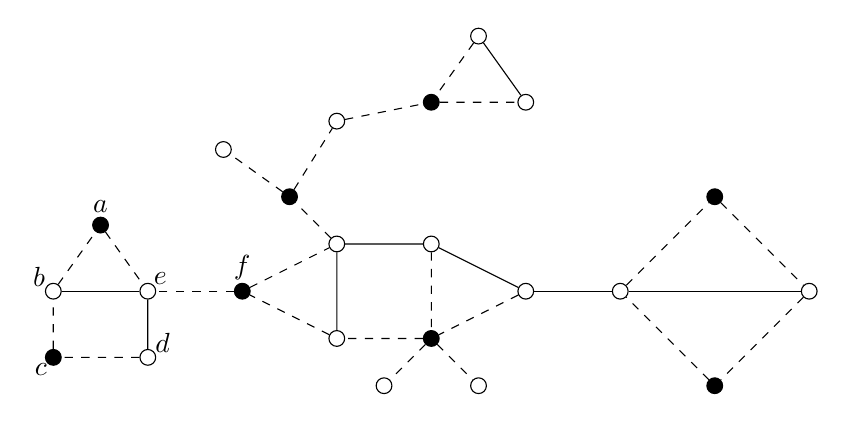
\begin{tikzpicture}[scale=1.2,auto=left]
    
    
    \begin{scope}[every node/.style={circle,draw=black,fill=white,minimum size=0.2cm, inner sep=0}]
      \node[fill=black,label=91:$f$] (a) at (0,0) {};
      \node[] (b) at (1,0.5) {};
      \node[] (c) at (2,0.5) {};
      \node[] (d) at (3,0) {};
      \node[fill=black] (e) at (2,-0.5) {};
      \node[] (f) at (1,-0.5) {};
      \node[] (g) at (4,0) {};
      \node[fill=black] (h) at (5,1) {};
      \node[] (i) at (6,0) {};
      \node[fill=black] (j) at (5,-1) {};
      \node[label=45:$e$] (k) at (-1,0) {};
      \node[label=45:$d$] (l) at (-1,-0.7) {};
      \node[fill=black,label=-135:$c$] (m) at (-2,-0.7) {};
      \node[label=135:$b$] (n) at (-2,0) {};
      \node[fill=black,label=90:$a$] (o) at (-1.5,0.7) {};
      \node[fill=black] (p) at (0.5,1) {};
      \node[] (q) at (-0.2,1.5) {};
      \node[] (r) at (1,1.8) {};
      \node[] (s) at (1.5,-1) {};
      \node[] (t) at (2.5,-1) {};
      
      \node[fill=black] (u) at (2,2) {};
      \node[] (v) at (3,2) {};
      \node[] (w) at (2.5,2.7) {};
      
      \foreach \from/\to in {b/c,c/d,f/b,
                             d/g,g/i,
                             k/l,k/n,
                             v/w}
	\draw (\from) -- (\to);

      \foreach \from/\to in {a/b,f/a,d/e,e/f,g/h,h/i,i/j,j/g,l/m,m/n,n/o,o/k,
                             b/p,p/q,p/r,c/e,e/t,e/s,a/k,r/u,u/v,w/u}
	\draw[dashed,black] (\from) -- (\to);
	
%      \foreach \from/\to in {a/p,p/h,j/e,a/o,p/u}
%	\draw[dashed,red] (\from) -- (\to);
	
%       \draw[dashed,red] (h) .. controls (7,1) and (7,-1) .. (j);
%       \draw[dashed,red] (e) .. controls (0.8,-1) .. (a);
%       \draw[dashed,red] (a) .. controls (-1,-1.2) .. (m);
%       \draw[dashed,red] (m) .. controls (-2.5,-0.2) and (-2.5,1) .. (o);
%       \draw[dashed,red] (p) .. controls (0,2) and (1.5,2.75) .. (u);
	
%       \draw[dotted] (u) .. controls (-0.5,2.5) and (1.7,2.2) .. (w);
%       
      
    \end{scope}
  \end{tikzpicture}
    \caption{Blocking set $B$ of an outerplane graph $G$, with blocking set vertices denoted in black. In dashed, edges of $G\setminus B$. Notice that, for each 2-connected component of $G$, the vertices of that component in $G\setminus B$ are contained in a single tree.}

  \label{fig:blocking_set}  
\end{figure}

The definition of a blocking set is subtle and implies three properties
that we will use throughout. A \emph{chord} in an outerplanar graph
is an edge that is not incident to the outer face.

\begin{obs}
   For any blocking set $B$ of $G$, $B$ does not include both endpoints
   of any chord of $G$.
\end{obs}

\begin{obs}
   For any blocking set $B$ of $G$ and any inner face $F$ of $G$, the
   vertices of $V(F)\cap B$ occur consecutively on the boundary of $F$ 
\end{obs}

\begin{obs}
  For every inner face $F$ of $G$, $F \setminus B$ is a non-empty path.
  \label{claim:facesMinusBarePaths}
\end{obs}
 

% Otherwise, removing $B$ would disconnect $F$ 

Let us now show that such a blocking set exists for all outerplane graphs. In fact, we will show something stronger:  we can pick any single vertex of $G$ and require it to be in the blocking set. This constraint will be crucial later.

\begin{lemma}
 Every outerplane graph $G$ has a blocking set. Moreover, if $G$ has
 $f\ge 1$ inner faces,  then given any vertex $v$ incident to some inner
 face $F_1$, there exists a blocking set $B$ of $G$ such that $v \in B$
 and for each inner face $F$ of $G$, $|V(F) \cap B|=1$.
 \label{lem:blocking_out}
\end{lemma}
\begin{proof}
 Let $F_1,F_2,\ldots,F_{f}$ be an ordering of the inner faces of $G$ such that $v \in V(F_1)$ and for each face $F_i$, $F_i$ shares an edge with at most one face in $\{F_1,\ldots,F_{i-1}\}$. Note that at most one edge can be shared by any two faces of an outerplane graph, otherwise a vertex would not be adjacent to the outer face. 
%  \begin{equation}
%   \bigl|\{ F_j \;|\; 1 \leq j < i \text{ and } E(F_j) \cap E(F_i)\not= \emptyset \}\bigr| \leq 1.
%  \end{equation}
 Such an ordering exists since $\wdual{G}$ is cycle-free. For each $i$, let $G_i$ be the graph induced by
 \begin{equation}
  \bigcup_{1 \leq j \leq i}V(F_j).
 \end{equation}
 We construct $B$ as follows: For $F_1$, set $B_1=\{v\}$. For each face $F_i$, $2 \leq i \leq f$, if $V(F_i) \cap B_{i-1} \not= \emptyset$, let $B_i = B_{i-1}$. Otherwise, select any vertex $v \in V(F_i) \setminus V(G_{i-1})$ and let $B_i = B_{i-1} \cup \{v\}$. Such a vertex exists since $|V(F_i) \cap V(G_{i-1})|\leq2$ and each face is incident to at least three vertices. We refer to the vertices in $V(F_i) \cap V(G_{i-1})$ as the \emph{anchors} of $F_i$. Recall that $B_f$ is the blocking set after considering all faces of $G$. Let $B=B_{f}$.
 
 \begin{claim}
  For each inner face $F_i$ of $G$, $|V(F_i) \cap B|=1$. Thus, $F_i \setminus B$ is a non-empty path.
  \label{claim:blocking_out_1}
 \end{claim}
 
 \begin{proof}
  We prove both sides of the equality:
  \begin{itemize}
   \item $|V(F_i) \cap B|\geq1$. This is true if $F_i=F_1$, and for $i \in \{2,\ldots,f\}$, we add a vertex of $F_i$ to $B_i$ if $V(F_i) \cap B_{i-1}=\emptyset$, so $|V(F) \cap B|\geq1$.
   \item $|V(F_i) \cap B|\leq1$. For each face $F_j$, $i < j \leq f$ subsequently visited, if $V(F_j) \cap B_{j-1} \not= \emptyset$, no other vertex is added, otherwise, a vertex not in $G_{j-1}\supseteq F_i$ is selected. Thus, $|V(F_i) \cap B|\leq1$. 
  \end{itemize}
  This completes the proof.
 \end{proof}
 
 \begin{claim}
  For each 2-connected component $H$ of $G$, $H\setminus B$ is connected.
  \label{claim:blocking_out_2}
 \end{claim}
 
 \begin{proof}
 Let $F_1^H,\ldots,F_{f_H}^H$ be the inner faces of $H$ in the order
 considered by the procedure. and let $G_i^H$ be the graph induced by  
 \begin{equation}
  \bigcup_{1 \leq j \leq i}V(F_j^H).
 \end{equation}
 We prove this by induction on $i$. Base case: $G_1^H=F_1^H$ is a cycle and by Claim \ref{claim:blocking_out_1} $|F_1^H \cap B|=1$, so $G_1^H\setminus B$ is a path, which is a connected graph. Induction step: suppose this holds for $G_{i-1}^H$. Let $B_{k-1}$ be the subset of $B$ that corresponds to all the faces visited prior to $F_i^H$. There are two cases:
 
 \begin{enumerate}
  \item $|B_{k-1} \cap V(F_i^H)|=1$. In this case, one of the anchors
  of $F_i^H$ is in $B_{k-1}$. Thus, since $F_i^H$ is a cycle, $F_i^H
  \setminus B$ is a path. This path is connected by the other anchor
  of $F_i^H$ to $G_{i-1}^H$, which is connected. Thus, $G_i^H$ is also
  connected. 
  \item $B_{k-1} \cap V(F_i^H) = \emptyset$. In this case, none of the
  anchors $a_1,a_2$ of $F_i^H$ are in $B_{k-1}$ and since $a_1,a_2 \in
  G_{i-1}^H$, $a_1,a_2 \notin B_k$. $F_i^H$ is a cycle, so by Claim
  \ref{claim:blocking_out_1}, $F_i^H \setminus B$ is a path which
  contains both $a_1$ and $a_2$. This path is connected to $G_{i-1}^H$,
  which is connected by the induction hypothesis, therefore $G_i^H$
  is also connected.
 \end{enumerate}
 This completes the proof.
 \end{proof}
 
 \begin{claim}
  For each 2-connected component $H$ of $G$, $H\setminus B$ is a tree.
  \label{claim:blocking_out_3}
 \end{claim}
 
 \begin{proof}
 Suppose $H\setminus B$ is not a tree. By Claim \ref{claim:blocking_out_2}, $H\setminus B$, is connected, therefore, $H\setminus B$ must contain a cycle. Let $C$ be the smallest such cycle. $C$ cannot correspond to some inner face $F$ of $H$, as by Claim \ref{claim:blocking_out_1}, $F \setminus B$ is a path. Therefore, since $H$ is outerplane, $H[C]$ must contain a chord. Therefore, $H[C]$ contains at least two simple cycles $C_1,C_2$ such that $C_1,C_2 \subset C \subseteq V(H) \setminus B$, which implies that both $C_1$ and $C_2$ are smaller than $C$. But, we chose $C$ to be the smallest such cycle. Contradiction. 
 \end{proof}
 
 \noindent This completes the proof of the lemma. 
\end{proof}

% Add a discussion about how this proves 8 for biconnected outerplane graphs
At this point we pause to sketch how Lemma~\ref{lem:blocking_out}
can already be used to give an upper-bound of 8 on the facial
non-repetitive chromatic number of biconnected outerplane graphs.
For a biconnected outerplane graph, $G$, we take a blocking set $B$
of $G$ using Lemma~X.  By Theorem~X, we can non-repetitively 4-colour the tree
$T=G\setminus B$ using the colours $\{1,2,3,4\}$, so what remains is to assign
colours to the vertices in $B$.  To do this, we use Theorem~X to non-repetitively 4-color
the cycle, $C$, that contains the vertices of $B$ in the order they appear on
the outer face of $G$ using the colours $\{5,6,7,8\}$.  We claim that
the resulting 8-colouring of $G$ is facially non-repetitive.  No facial
path on an interior face is coloured repetitively since each such facial path
is also either present in the tree $T$ or it contains exactly one
vertex of $B$.  No facial path on the outer face is coloured repetitively
since it is obtained by interleaving a non-repetitive sequence of colours in $C$ with non-repetive sequences taken from $T$; by Lemma~X, a sequence obtained in this way is non-repetitive.

In Section~\ref{sec:X}, we show that the preceding argument can be
improved to give a bound of 7 on the facial non-repetitive chromatic
number of biconnected outerplane graphs. This is just a matter of adding
vertices to the blocking set so that the cycle $C$ does not have length
in $\{\}$, so that it can non-repetitively 3-coloured. 
\begin{corollary}
 Let $G$ be a 2-connected outerplane graph that contains at least two inner faces. There exists a blocking set $B$ of $G$ such that for each inner face $F$ of $G$, $|V(F) \cap B|=1$, and there exists an inner face $F_1$ of $G$ with $\deg_{\wdual{G}}(F_1)=1$ such that the vertex $v \in V(F_1) \cap B$ has $\deg_G(v) \geq 3$.
  \label{cor:blocking_out_select}
\end{corollary}

\begin{proof}
  Pick a face $F_1$ such that $\deg_{\wdual{G}}(F_1)=1$ and a vertex $v \in V(F_1)$ such that $\deg_G(v) \geq 3$. Such a vertex exists since $G$ is 2-connected and contains at least two inner faces. Lemma \ref{lem:blocking_out} completes the proof. 
\end{proof}

\subsection{Colouring Outerplane Graphs}

We will now show how to use a blocking set to get a facial nonrepetitive
colouring of an outerplane graph. Let $G$ be an outerplane graph and $B$
be a blocking set of $G$. 

The \emph{blocking graph} of $G$ for a blocking set $B$ is the graph
whose vertex set is $B$ and whose edges are defined as follows:  Begin
with the facial walk $W$ on the outer face of $G$. Remove every vertex
 not in $B$ from $W$ to obtain a cyclic sequence $W'$ of vertices in
$B$. For each consecutive pair of vertices $uw$ in $W'$ we add the edge
 $uw$ to the blocking graph.  This naturally defines the embedding of
 the blocking graph $\block_B(G)$. See Figure~\ref{fig:blocking_graph}
 for an example.   Note that $\block_B(G)$ is not necessarily a simple
graph; it may contain parallel edges (cycles of length two) and self-loops
(cycles of length one). 
\begin{figure}[!ht]
  \centering
  
  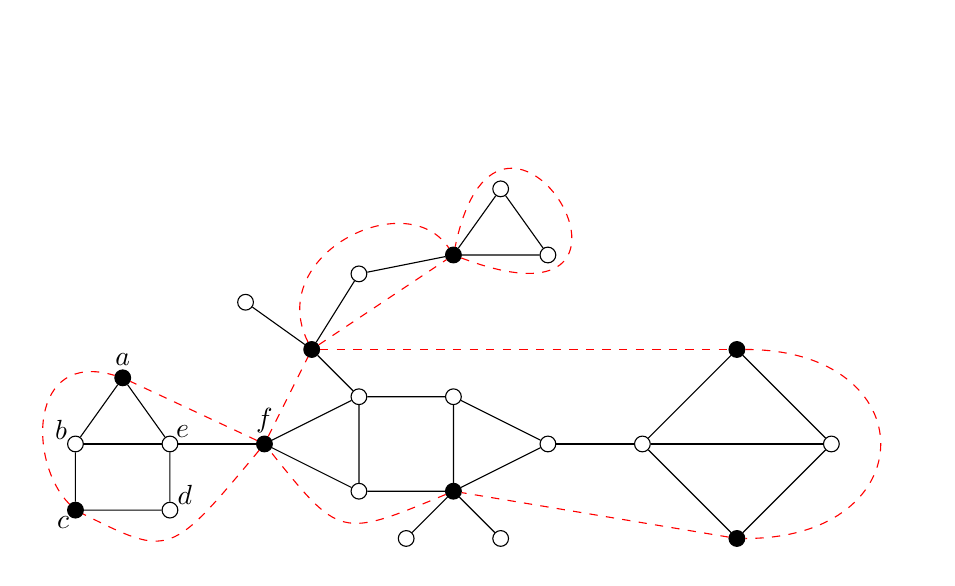
\begin{tikzpicture}[scale=1.2,auto=left]
    
%     \node[style={text=black}] at (-1.5,0) {$H$};
    
    \begin{scope}[every node/.style={circle,draw=black,fill=white,minimum size=0.2cm, inner sep=0}]
      \node[fill=black,label=91:$f$] (a) at (0,0) {};
      \node[] (b) at (1,0.5) {};
      \node[] (c) at (2,0.5) {};
      \node[] (d) at (3,0) {};
      \node[fill=black] (e) at (2,-0.5) {};
      \node[] (f) at (1,-0.5) {};
      \node[] (g) at (4,0) {};
      \node[fill=black] (h) at (5,1) {};
      \node[] (i) at (6,0) {};
      \node[fill=black] (j) at (5,-1) {};
      \node[label=45:$e$] (k) at (-1,0) {};
      \node[label=45:$d$] (l) at (-1,-0.7) {};
      \node[fill=black,label=-135:$c$] (m) at (-2,-0.7) {};
      \node[label=135:$b$] (n) at (-2,0) {};
      \node[fill=black,label=90:$a$] (o) at (-1.5,0.7) {};
      \node[fill=black] (p) at (0.5,1) {};
      \node[] (q) at (-0.2,1.5) {};
      \node[] (r) at (1,1.8) {};
      \node[] (s) at (1.5,-1) {};
      \node[] (t) at (2.5,-1) {};
      
      \node[fill=black] (u) at (2,2) {};
      \node[] (v) at (3,2) {};
      \node[] (w) at (2.5,2.7) {};
      
      \foreach \from/\to in {a/b,b/c,c/d,d/e,e/f,f/a,f/b,c/e,
                             d/g,g/h,h/i,i/j,j/g,g/i,
                             a/k,k/l,l/m,m/n,n/o,o/k,k/n,
                             e/t,e/s,  b/p,p/q,p/r,
                             r/u,u/v,v/w,w/u}
	\draw (\from) -- (\to);
	
      \foreach \from/\to in {a/p,p/h,j/e,a/o,p/u}
	\draw[dashed,red] (\from) -- (\to);
	
       \draw[dashed,red] (h) .. controls (7,1) and (7,-1) .. (j);
       \draw[dashed,red] (e) .. controls (0.8,-1) .. (a);
       \draw[dashed,red] (a) .. controls (-1,-1.2) .. (m);
       \draw[dashed,red] (m) .. controls (-2.5,-0.2) and (-2.5,1) .. (o);
       \draw[dashed,red] (p) .. controls (0,2) and (1.5,2.75) .. (u);

       \draw[dashed,red] (u) .. controls (4.5,1.05) and (2.5,4.4) .. (u);
	
%       \draw[dotted] (u) .. controls (-0.5,2.5) and (1.7,2.2) .. (w);
%       
      
    \end{scope}
  \end{tikzpicture}
  
  \caption{An outerplane graph $G$ with blocking set $B$ (denoted in black). The edges of $\block_{B}(G)$ are denoted in dashed. Vertices $a,b,c,d,e,f$ induce a spider graph $H$}
  \label{fig:blocking_graph}
  
  \end{figure}

In the previous section, we sketched a proof of an upper bound of 8 on the facial chromatic number of biconnected outerplane graphs.  This proof works by non-repetitively 4-colouring the tree, $G\setminus B$, obtained after removing the blocking set and then non-repetiviely 4-colouring a cycle, $C$, of vertices in the blocking set.  This cycle, $C$, is actually the blocking graph, $\block_B(G)$.  The following lemma shows that this strategy generalizes to the situation where we can find a facial non-repetitive colouring of $\block_B(G)$ with few colours.


%\begin{figure}
%  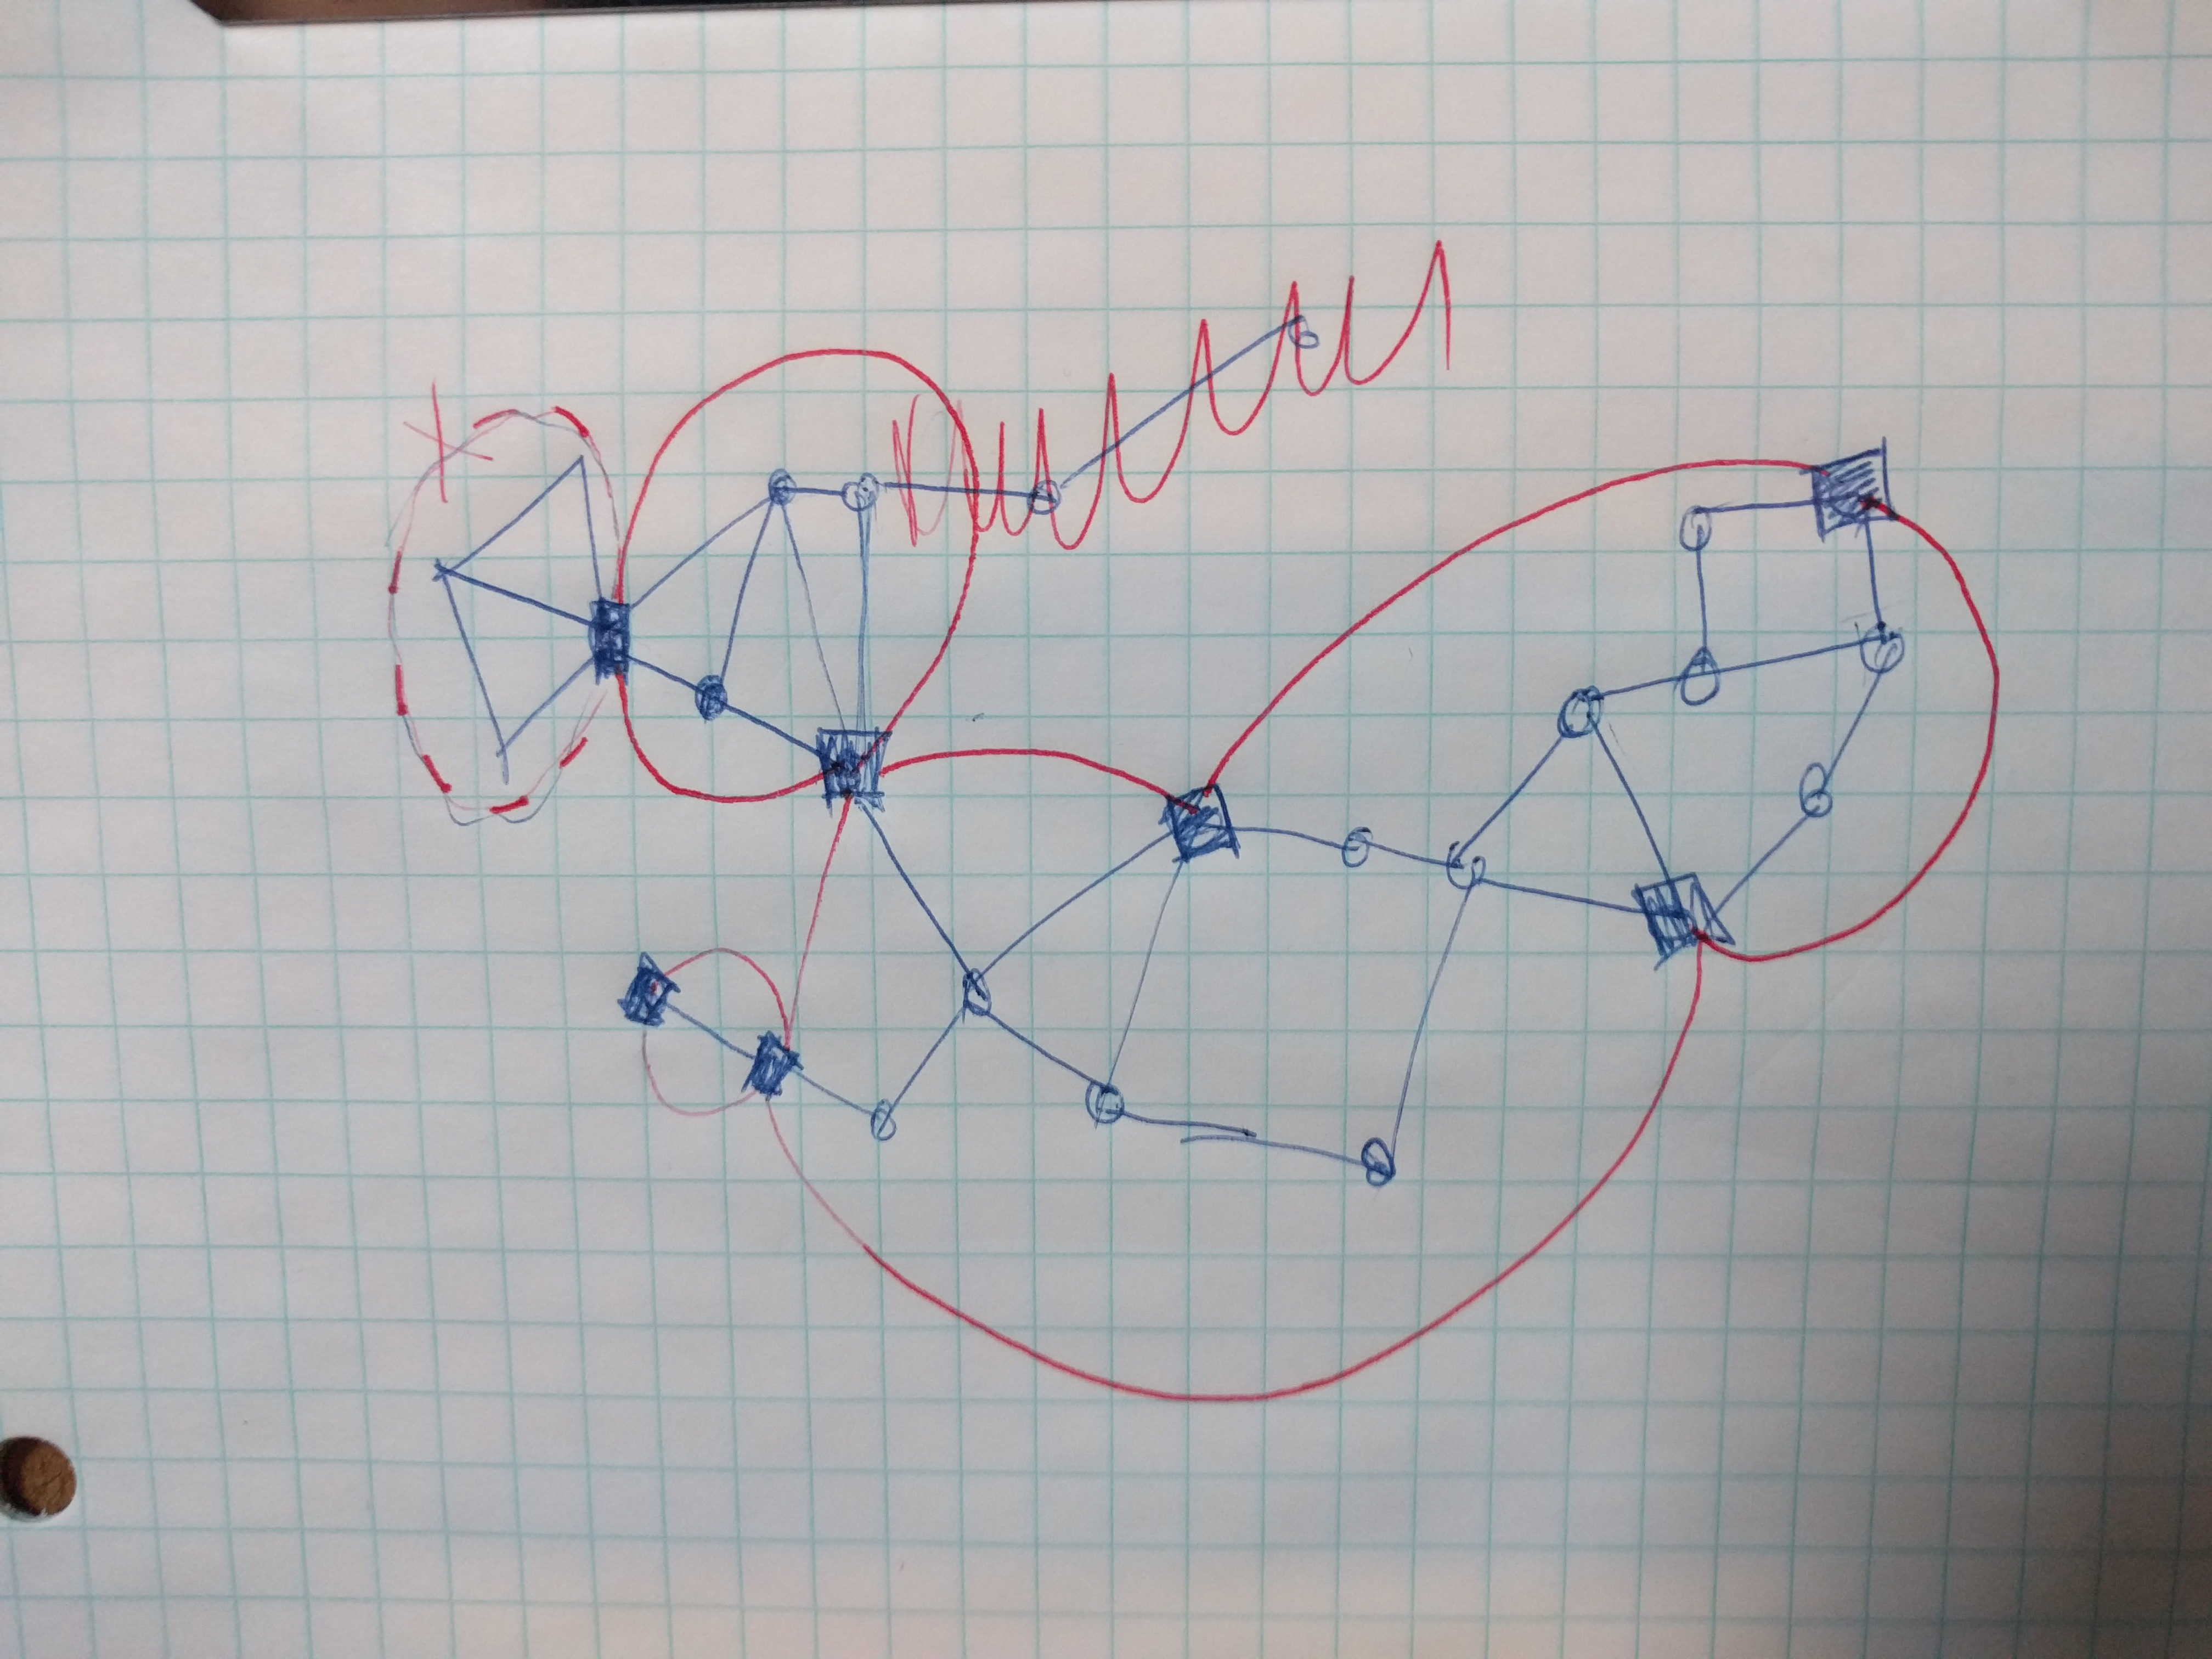
\includegraphics[width=.9\textwidth]{images/blocking}
%  \caption{An example of a blocking graph}
%  \label{fig:blocking-graph}
%\end{figure}
%
%A \emph{blocking graph} of $G$ is a (simple)
%graph denoted by $\block_{B}(G)$ with vertex set $B$ and with an edge
%set defined as follows: Let $W=w_1,w_2,\ldots,w_k$ be a closed facial
%walk around the outer face of $G$ such that $w_1=w_k\in B$. For each
%subsequence $w_i,w_{i+1},\ldots,w_{i+r}$ such that 

%\begin{enumerate}[a)]
% \item $w_i,w_{i+1},\ldots,w_{i+r}$ is a facial path,
% \item $r>0$,
% \item $w_i,w_{i+r}\in B$ and
% \item $w_{i+j}\notin B$ for all $j \in \{1, \ldots, r-1\}$,
%\end{enumerate}
%add an edge $\{w_i, w_{i+r}\}$ to $E(\block_{B}(G))$. 
%Thus, every pair of vertices of $B$ connected by a facial path on the outside face of $G$ are connected by an edge in $\block_{B}(G)$ (see Figure \ref{fig:blockingsetex}). If we remove condition (a) (thus also adding edges between vertices connected together via a facial walk that contains repeated vertices), the resulting graph is called the \emph{augmented blocking graph}, and denoted $\block_{B}^+(G)$.
%
%$\block_{B}(G)$ is a minor of $G$, thus it is also an outerplane graph. Furthermore, since edges only link successive vertices on $W$, $\block_{B}(G)$ is chordless. A graph where every cycle is chordless is called a \emph{cactus graph}.\footnote{The most common definition says that a cactus graph is a graph in which any two simple cycles have at most one vertex is common. This is equivalent to a chordless graph.}
%

%\begin{figure}[!ht]
%  \centering
%  
%  \begin{tikzpicture}[scale=1.5,auto=left]
%        
%    \begin{scope}[every node/.style={circle,draw=black,fill=white,minimum size=0.2cm, inner sep=0}]
%      \node[fill=black,label=90:$a$] (a) at (0,1) {};
%      \node[] (b) at (1,1) {};
%      \node[fill=black,label=90:$b$] (c) at (2,1) {};
%      \node[] (d) at (0,0) {};
%      \node[] (e) at (1,0) {};
%      \node[] (f) at (2,0) {};
%      \node[] (g) at (-1,1) {};
%      \node[fill=black,label=-90:$c$] (h) at (3,0) {};
%      \node[] (i) at (3.5,0) {};
%      \node[] (j) at (3,0.5) {};
%      \node[label=-180:$d$] (k) at (-1,0) {};
%      
%      \foreach \from/\to in {a/b,b/c,c/f,a/g,a/d,f/h,h/i,h/j}
%	\draw (\from) -- (\to);
%	
%      \foreach \from/\to in {d/g,d/e,e/f,e/b,i/j,d/k}
%	\draw[] (\from) -- (\to);
%	
%    \end{scope}
%  
%       \draw[dashed,red] (a) .. controls (0.2,1.2) and (1.8,1.2) .. (c); 
%       \draw[dashed,red] (c) -- (h);
%  \end{tikzpicture}
%  
%    \caption{The blocking graph has the blocking set as vertex set, and an edge between each pair of vertices that are connected through a facial path (dashed). There is no $\{a,c\}$ edge since there is no facial path between them that does not include another blocking set vertex. However, were $d$ not in the graph, the $\{a,c\}$ edge would exist.}
%
%  \label{fig:blockingsetex}  
%\end{figure}

\begin{lemma}
  Let $G$ be an outerplane graph and $B$ be a blocking set of
  $G$. Suppose that there exists a facial nonrepetitive $k$-colouring
  of $\block_{B}(G)$. Then, there exists a facial nonrepetitive
  $(4+k)$-colouring of $G$.
 \label{lem:hitting_plus_four}
\end{lemma}

%Note that this claim is different from Claim \ref{claim:blocking_out_1} since a blocking set may contain multiple vertices of a same inner face (which will happen in a later proof), while Lemma \ref{lem:blocking_out} shows the existence of a blocking set with exactly \emph{one} vertex per inner face.
 
% \begin{claim}
%  For every inner face $F$ of $G$, $F \setminus B$ is a non-empty path.
%  \label{claim:facesMinusBarePaths}
% \end{claim}
% 
% \begin{proof}
% Suppose that this is not the case, thus since $F \setminus B \not= \emptyset$, there exists an inner face $F$ where $F \setminus B$ consists at least two connected components. Let $H$ be the 2-connected component of $G$ that contains $F$. Let $u,v \in V(F) \cap B$ such that $u \not= v$ and $\{u,v\} \notin E(F)$. Two such vertices certainly exist since $F \setminus B$ consists at least two connected components. Let $H'=H \setminus \{u\}$. $v$ is a cut vertex of $H'$ since $F$ is a cycle, $H'$ is an outerplane graph and $u$ and $v$ are not adjacent. Thus, since $\{u,v\} \subseteq B$, $H \setminus B$ is not connected. But, by definition of a blocking set, $H \setminus B$ must be connected. Contradiction. 
% \end{proof} 
\begin{proof}
 Since $B$ is a blocking set of $G$, $G'=G \setminus B$ is a forest and by Theorem \ref{thm:four_colouring_trees}, there exists a nonrepetitive 4-colouring of each connected component of $G'$, which translates to a nonrepetitive 4-colouring of $G'$. Let $c_{G'} : V(G') \rightarrow \{1,2,3,4\}$ be such a colouring, and let $c_B : B \rightarrow \{5,\ldots,4+k\}$ be a facial nonrepetitive $k$-colouring of $\block_{B}(G)$. Such a colouring exists by our hypothesis. Let $c : V(G) \rightarrow \{1,\ldots,4+k\}$ be a $(4+k)$-colouring of $G$ defined as
 \begin{equation}
 c(v) = \begin{cases}
         c_B(v) \text{ if } v \in B\\
         c_{G'}(v) \text{ otherwise}.
        \end{cases}
 \end{equation}
 We now show that $c$ is a facial nonrepetitive colouring of $G$. Suppose that this is not the case. Thus, there exists a path $P$ on some face of $G$ such that the colour sequence of consecutive vertices of $P$ is a repetition. If $P$ is also a path on $G'$, then its colour sequence cannot be repetitive since $G'$ is nonrepetitively coloured under $c_G$, and by extension, under $c$. Thus, $P$ is not a path on $G'$. By the same reasoning, $P$ cannot be a path on $\block_{B}(G)$. Thus, $P$ alternates between vertices in $G'$ and vertices in $B$. 
 
 If $P$ is on an inner face $F$ of a 2-connected component $H$ of $G$, then by Claim \ref{claim:facesMinusBarePaths}, $P'=F \setminus B$ is a non-empty path on $F$. This implies that $P''=F\cap B$ is also a path --- on at least one vertex --- which lays on a face of $\block_{B}(G)$ by definition of the blocking graph since $P'$ is a path. Furthermore, by the respective colourings of $\block_B(G)$ and $G'$, $P$ and $P'$ will be nonrepetitive. Since $P$ is repetitive and the intersection of the domains of $c_G$ and $c_B$ is empty, $P$ must contain a block of the form $X_1,Y_1,X_2,Y_2$ where $X_1,X_2$ are vertices of $V(G')$ (or $B$) and $Y_1,Y_2$ are vertices of $B$ (or $V(G')$ respectively) and none of $X_1,X_2,Y_1,Y_2$ are empty. But, observe that this contradicts our claim that $P'$ and $P''$ are paths and, joined together, form a cycle --- $F$.
 
 Therefore, $P$ is on the outer face of $G$. Let $P'$ be the sequence of vertices of $P\cap B$ in the same order as in $P$. Observe that $P'$ will be a path in $\block_{B}(G)$. Thus, the colour sequence of $P'$ is nonrepetitive. Furthermore, each subsequence of consecutive vertices on $G'$ of $P\cap G'$ will also be nonrepetitive by the colouring of $G'$. Hence, by Lemma \ref{lem:nonrep_alternate}, $P$ is nonrepetitive. But this contradicts our assumption that $P$ is repetitive. This completes the proof.
\end{proof}

%Notice that the blocking graph of an outerplane graph with exactly one
%2-conn\-ected component is a cycle if $|B|\geq 3$ (otherwise it is a
%path on 1 or 2 vertices). Since every cycle or path has a nonrepetitive
%colouring with at most four colours, this implies the existence of a
%facial nonrepetitive 8-colouring of any such outerplane graph. We will
%later show how to tighten this bound to 7.

\subsection{Colouring Blocking Graphs}

We now show how to colour the blocking graph---a cactus graph---of an outerplane graph with at least two 2-connected components.
By Lemma \ref{lem:hitting_plus_four}, if we can find a facial nonrepetitive $k$-colouring of any cactus graph, we can get a facial nonrepetitive $k+4$-colouring of any outerplane graph. 

The tightest upper bound for the facial Thue chromatic number of outerplane graphs is 12, which is the bound for the Thue chromatic number \cite{barat2007square, kundgen2008nonrepetitive}. Thus, to improve this bound, we need to find a facial nonrepetitive 7-colouring of the blocking graph.  We have been unable to do this for general cactus graphs and we only have a solution for the case where all cycles of the cactus graph are even. 

We will address these difficulties by choosing a blocking set such that the blocking graph has no odd cycle. We will show how to achieve this in Lemma \ref{lem:cycle_spider_even}. 
A \emph{levelling} of a graph $G$ is a function $\lambda : V(G) \rightarrow \integers$ such that for each $\{u,v\}\in E(G)$, $|\lambda(u)-\lambda(v)|\leq 1$. The level pattern of a path $v_1,\ldots,v_k$ is the sequence $\lambda(v_1),\lambda(v_2),\ldots,\lambda(v_k)$.

\begin{lemma}[K{\"u}ndgen and Pelsmajer \cite{kundgen2008nonrepetitive}]
 Let $G$ be a graph and $\lambda$ be a levelling of $G$. Let $S=s_0,s_1,\ldots,s_m$ be a nonrepetitive palindrome-free sequence on an alphabet $\mathcal{A}$ with $m=\max\{\lambda(v) \;|\; v \in V(G)\}$ and $c : V(G) \rightarrow \mathcal{A}$ be a colouring of $G$ defined as $c(v)=s_{\lambda(v)}$. %Thus each $v \in V(G)$ gets the colour corresponding to its level, thus let . 
 If a path $P=P_1, P_2$ with $|P_1|=|P_2|$ in $G$ is repetitively coloured under $c$, then $P_1$ and $P_2$ have the same level pattern.
 \label{lem:level_pattern_palindrome_free}
\end{lemma}


\begin{lemma}
 %Let $\pi_o(G)$ be the minimum number of colours required for the outer face of a plane graph $G$ to be coloured nonrepetitively. 
 Let $G$ be a plane cactus graph such that every cycle of $G$ is even. Then, $\pi_f(G) \leq 7$.
 \label{lem:outer_face_cactus}
\end{lemma}

\begin{proof}
 We may assume that $G$ is connected as this does not affect its facial Thue chromatic number. Also, assume that $G$ is neither a cycle nor a tree since $\pi_f(G) \leq 4 < 7$ for both these classes of graphs.  
 If there exists a vertex $v$ of $G$ such that $\deg_G(v)=1$, then let the \emph{root} $r$ of $G$ be $v$. Otherwise, let $r$ be any vertex of $G$. Let $\lambda$ be a levelling of $G$ defined as $\lambda(v) = \dist(r,v)$. Let $H$ be a graph that contains all vertices $v\in V(G)$ such that
 \begin{enumerate}[a)]
  \item $v$ is on a cycle $C$ of $G$,
  \item $\lambda(v)=\max_{u \in C} \lambda(u)$ and
  \item $\deg_G(v)=2$.
 \end{enumerate} 
 In other words, $H$ contains the vertices of degree 2 that are on the deepest level of a cycle (see Figure \ref{fig:adding_vertices_H}). Notice that since every cycle of $G$ is even, there is at most one vertex of $H$ in each cycle of $G$. If $\deg_G(r)\not=1$, there must exist at least one face $F_T$ of $G$ such that exactly one vertex $v$ of $F_T$ has degree greater than two (otherwise, since $G$ is neither a cycle nor a tree and is connected, there would be infinitely many faces in $G$). Since all faces of $G$ are even and $G$ does not contain double edges, $F_T$ contains at least three vertices of degree 2, say $a,b,c$. Without loss of generality, assume that $a \in V(H)$. If $|V(H)|\in \{5,7,10,14,17\}$, add $b$ to $V(H)$. If $|V(H)|=9$, add both $b$ and $c$ to $V(H)$. Notice that now, either $\deg_G(r)=1$ or $|V(H)|\notin \{5,7,9,10,14,17\}$.
 
 \begin{figure}  
  \centering
  
  \begin{subfigure}[t]{0.45\textwidth}
    \centering
    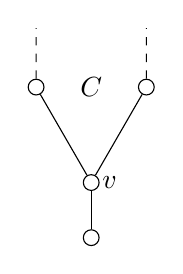
\begin{tikzpicture}[scale=1.4,auto=left]
	
    \node at (0,0.866) {$C$};
    
      \begin{scope}[every node/.style={circle,draw=black,fill=white,minimum size=0.2cm, inner sep=0}]

	\node[label=0:$v$] (a) at (0,0) {};
	\node[] (b) at (-0.5,0.866) {};
	\node[] (c) at (0.5,0.866) {};
	\node[] (d) at (0,-0.5) {};
	
	\foreach \from/\to in {a/b,a/c,a/d}
	  \draw (\from) -- (\to);  
	  
	  \draw[dashed] (b) -- (-0.5,1.4);
	  \draw[dashed] (c) -- (0.5,1.4);
	
      \end{scope}
    \end{tikzpicture}
    \caption{$v$ has degree greater than 2, so it is not in $H$}   
  \end{subfigure}
  ~
  \begin{subfigure}[t]{0.45\textwidth}
    \centering  
    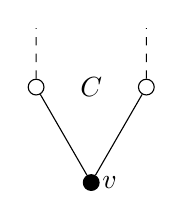
\begin{tikzpicture}[scale=1.4,auto=left]    
      \node at (0,0.866) {$C$};
	  
      \begin{scope}[every node/.style={circle,draw=black,fill=white,minimum size=0.2cm, inner sep=0}]

	\node[fill=black,label=0:$v$] (a) at (0,0) {};
	\node[] (b) at (-0.5,0.866) {};
	\node[] (c) at (0.5,0.866) {};
	
	\foreach \from/\to in {a/b,a/c}
	  \draw (\from) -- (\to);  
	  
	  \draw[dashed] (b) -- (-0.5,1.4);
	  \draw[dashed] (c) -- (0.5,1.4);
	
      \end{scope}
    \end{tikzpicture}
    \caption{$v$ has degree 2, so it is in $H$}
  \end{subfigure}

  \caption{Adding vertices to $H$.}
  \label{fig:adding_vertices_H}
  
\end{figure}  
 
 \begin{figure}[!ht]
  \centering
  
  \begin{subfigure}[b]{0.45\textwidth}
  \centering
  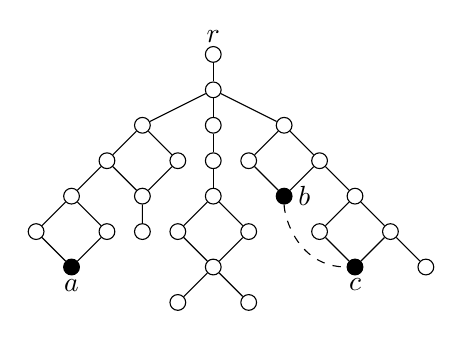
\begin{tikzpicture}[scale=0.9,auto=left]
        
    \begin{scope}[every node/.style={circle,draw=black,fill=white,minimum size=0.2cm, inner sep=0}]
%       \node[fill=black,label=-90:$f$] (a) at (0,0) {};

      \node[label=90:$r$] (root) at (0,0.5) {};
      \node[] (a) at (0,0) {};
      \node[] (b) at (-1,-0.5) {};
      \node[] (c) at (1,-0.5) {};
      \node[] (d) at (-1.5,-1) {};
      \node[] (e) at (-0.5,-1) {};
      \node[] (f) at (0.5,-1) {};
      \node[] (g) at (1.5,-1) {};
      \node[] (h) at (-2,-1.5) {};
      \node[] (i) at (-1,-1.5) {};
      \node[fill=black,label=0:$b$] (j) at (1,-1.5) {};
      \node[] (k) at (2,-1.5) {};
      \node[] (l) at (-2.5,-2) {};
      \node[] (m) at (-1.5,-2) {};
      \node[] (n) at (-1,-2) {};
      \node[] (o) at (1.5,-2) {};
      \node[] (p) at (2.5,-2) {};
      \node[fill=black,label=-90:$a$] (q) at (-2,-2.5) {};
      \node[fill=black,label=-90:$c$] (r) at (2,-2.5) {};
      \node[] (s) at (3,-2.5) {};
      \node[] (t) at (0,-0.5) {};
      \node[] (u) at (0,-1) {};
      \node[] (v) at (0,-1.5) {};
      \node[] (w) at (-0.5,-2) {};
      \node[] (x) at (0.5,-2) {};
      \node[] (y) at (0,-2.5) {};
      \node[] (z1) at (-0.5,-3) {};
      \node[] (z2) at (0.5,-3) {};
      
      \foreach \from/\to in {a/b,a/c,b/d,b/e,e/i,c/f,c/g,d/h,d/i,f/j,g/j,g/k,h/l,h/m,i/n,k/o,k/p,l/q,m/q,o/r,p/r,p/s,
			     a/t,t/u,u/v,v/w,v/x,w/y,x/y,y/z1,y/z2,root/a}
	\draw (\from) -- (\to);   
	
       \draw[dashed,black] (j) .. controls (1,-1.8) and (1.2,-2.5) .. (r);    
      
    \end{scope}
  \end{tikzpicture}
  \end{subfigure}
  ~
  \begin{subfigure}[b]{0.5\textwidth}
  \centering
  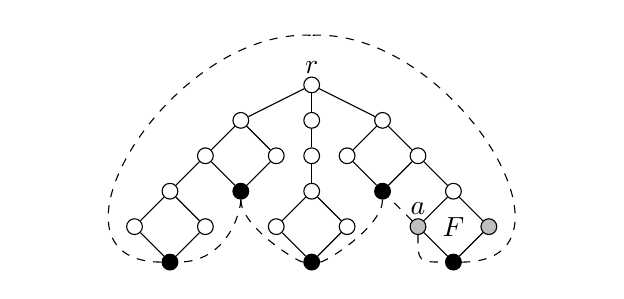
\begin{tikzpicture}[scale=0.9]
  
    \node[] at (2,-2) {$F$};
        
    \begin{scope}[every node/.style={circle,draw=black,fill=white,minimum size=0.2cm, inner sep=0}]
%       \node[fill=black,label=-90:$f$] (a) at (0,0) {};

      \node[label=90:$r$] (a) at (0,0) {};
      \node[] (b) at (-1,-0.5) {};
      \node[] (c) at (1,-0.5) {};
      \node[] (d) at (-1.5,-1) {};
      \node[] (e) at (-0.5,-1) {};
      \node[] (f) at (0.5,-1) {};
      \node[] (g) at (1.5,-1) {};
      \node[] (h) at (-2,-1.5) {};
      \node[fill=black] (i) at (-1,-1.5) {};
      \node[fill=black] (j) at (1,-1.5) {};
      \node[] (k) at (2,-1.5) {};
      \node[] (l) at (-2.5,-2) {};
      \node[] (m) at (-1.5,-2) {};
%       \node[] (n) at (-1,-2) {};
      \node[fill=lightgray,label=90:$a$] (o) at (1.5,-2) {};
      \node[fill=lightgray] (p) at (2.5,-2) {};
      \node[fill=black] (q) at (-2,-2.5) {};
      \node[fill=black] (r) at (2,-2.5) {};
      \node[] (t) at (0,-0.5) {};
      \node[] (u) at (0,-1) {};
      \node[] (v) at (0,-1.5) {};
      \node[] (w) at (-0.5,-2) {};
      \node[] (x) at (0.5,-2) {};
      \node[fill=black] (y) at (0,-2.5) {};
      
      \foreach \from/\to in {a/b,a/c,b/d,b/e,e/i,c/f,c/g,d/h,d/i,f/j,g/j,g/k,h/l,h/m,k/o,k/p,l/q,m/q,o/r,p/r,
			     a/t,t/u,u/v,v/w,v/x,w/y,x/y}
	\draw (\from) -- (\to);   
	
       \draw[dashed,black] (o) -- (j);  
       \draw[dashed,black] (o) .. controls (1.5,-2.5) .. (r);   
       \draw[dashed,black] (j) .. controls (1,-2) and (0.2,-2.5) .. (y);    
       \draw[dashed,black] (i) .. controls (-1,-2) and (-0.2,-2.5) .. (y);  
       \draw[dashed,black] (i) .. controls (-1,-1.8) and (-1.2,-2.5) .. (q);   
       
       \draw[dashed,black] (q) .. controls (-4,-2.5) and (-2,0.8) .. (0,0.7);  
       \draw[dashed,black] (r) .. controls (4,-2.5) and (2,0.8) .. (0,0.7);  
      
    \end{scope}
  \end{tikzpicture}
  \end{subfigure}
  
  \caption{Two examples of cactus graphs and their levellings ($r$ is at level 0). In black: vertices of $H$, with the edges of $H$ represented in black.
  Left: There is at least one vertex of degree 1, which becomes the root. Notice there is no edge between $a$ and $b$ since the facial walk between them contains vertices of degree 1, but this is not the case between $b$ and $c$. Right: No such vertex exists, but there is at least one face ($F$ in this example) in which two additional vertices can be added. Here, since $|V(H)|=5$, one vertex ($a$, in gray), was added to $H$.}
  \label{fig:colouring_cactus}
 \end{figure}

 
 We now define the edge set $E(H)$ of $H$. Let $W$ be a closed facial walk around the outer face of $G$. Note that since they have degree two and are on cycles, vertices in $H$ appear exactly once in $W$. Add an edge between any two vertices $u,v \in V(H)$ if and only if 
 \begin{enumerate}[a)]
  \item $u,v_1,v_2,\ldots,v_k,v$ is a walk in $W$,
  \item for each $v_i$, $\deg_G(v_i) > 1$ and $v_i \notin V(H)$
  \item $u\not=v$.
 \end{enumerate}
 Note that $H$ is either a cycle or a forest of paths (the latter possibly empty or a single connected component), see Figure \ref{fig:colouring_cactus}. Let $\mathcal{A}$ and $\mathcal{B}$ be two disjoint colour sets. Let $h=\max_{v \in V(G)} \lambda(v)$ and $S=s_0,s_1,\ldots,s_h$ be a palindrome-free nonrepetitive sequence on $\mathcal{A}$. Let $c_H : V(H) \rightarrow \mathcal{B}$ be a nonrepetitive colouring of $H$. We define a colouring $c : V(G) \rightarrow \mathcal{A} \cup \mathcal{B}$ as follows:
 \begin{equation}
  c(v) = \begin{cases}
          c_H(v) & \text{ if } v \in V(H)\\
          s_{\lambda(v)} & \text{ otherwise.}
         \end{cases}
 \end{equation}
 We will now show that $c$ is a valid nonrepetitive colouring of $G$. Suppose that this is not the case. Thus, there exists a path $P=P_1,P_2$ such that the colour sequence $S$ corresponding to vertices of $P$ is a repetition. Let us first suppose that $P$ is on the outer face of $G$. We will need the following claim:
 
 \begin{claim}
  Let $P$ be a path on the outer face of $G$ such that $P \cap V(H) = \emptyset$. The level sequence $L$ corresponding to vertices of $P$ must be strictly decreasing, strictly increasing, or strictly decreasing then strictly increasing.
  \label{claim:strictly_inc_dec}
 \end{claim}
 \begin{proof}
 Suppose that this is not the case. $L$ cannot contain a block of the form $i,i$ as this can only correspond to an odd cycle of $G$, but all cycles of $G$ are even. Thus, $L$ must contain a block of the form $i,i+1,i$. Since $P$ is on the outer face, we must have that the vertex $v$ corresponding to $i+1$ is the lowest vertex on some cycle $C$ and that $\deg_G(v)=2$. But in this case, $v$ must be in $H$, which is a contradiction. 
 \end{proof}
 By Lemma \ref{lem:level_pattern_palindrome_free}, $P_1$ and $P_2$ have the same level pattern. However, if $P \cap V(H) = \emptyset$ this is incompatible with Claim \ref{claim:strictly_inc_dec} which states that the level sequence of $P$ must be strictly decreasing, strictly increasing, or strictly decreasing then strictly increasing.  Thus, $P$ must contain vertices of $H$. Let $P_H=p_1,p_2,\ldots,p_k$ be the sequence of vertices of $P \cap V(H)$ in the same order as in $P$. Notice that we must have $\{p_i,p_{i+1}\}\in E(H)$ for each $1 \leq i < k$ as this corresponds to the definition of an edge in $H$. Therefore, the colour sequence corresponding to $P_H$ must be nonrepetitive. Since vertices on $G\setminus{H}$ and vertices on $H$ are coloured with $\mathcal{A}$ and $\mathcal{B}$ respectively, and $\mathcal{A} \cap \mathcal{B} = \emptyset$, then by Lemma \ref{lem:nonrep_alternate}, the colour sequence of vertices in $P$ is nonrepetitive as well. 
 
 Thus, $P$ must be on some inner face $F$ of $G$. With the exception of $F_T$ (if it exists), all inner faces of $G$ contain at most one vertex in $H$. If $P\cap V(H) \not= \emptyset$, then since $\mathcal{A} \cap \mathcal{B} = \emptyset$, we must have that $F=F_T$. Let $P_H=p_1,\ldots,p_k$ be the sequence of vertices of $P \cap V(H)$ in the same order as in $P$. Since all the vertices of $P_H$ are on the same inner face and $F_T$ has exactly one vertex of degree greater than three, $\{p_i,p_{i+1}\}\in E(H)$ for each $1 \leq i < k$. Thus, using the same argument as in the previous case, the colour sequence of vertices in $P$ must be nonrepetitive. 
 
 Therefore, $P \cap V(H) = \emptyset$. Again, by Lemma \ref{lem:level_pattern_palindrome_free}, $P_1$ and $P_2$ have the same level pattern. But, since $P$ is constrained to $F$, whose level sequence is circular, $P_1$ and $P_2$ cannot have the same level pattern unless $P$ contains duplicate vertices. Therefore, $c$ is a valid nonrepetitive facial colouring of $G$.
 
 It now remains to show that $|\mathcal{A}|+|\mathcal{B}|=7$. A nonrepetitive palindrome-free sequence can be constructed from any ternary nonrepetitive sequence by adding a fourth symbol between blocks of size 2 \cite{brevsar2007nonrepetitive}. Thus, four symbols are sufficient for $\mathcal{A}$. Notice that $H$ is a cycle if and only if $\deg_G(r)\not=1$. In this case, we made sure that $|V(H)| \notin \{5,7,9,10,14,17\}$. Such a cycle has a nonrepetitive 3-colouring by Theorem \ref{thm:colouring_cycles}. Otherwise, it is a forest of paths, for which three symbols are also sufficient by Thue's original result. This completes the proof. 	
\end{proof}


\subsection{Even Cycles}
Let us now show how to construct a blocking set, $B$, for an outerplane graphs, $G$,
so that every cycle of $\block_B(G)$ is even. 

% A \emph{spider graph} is a connected outerplane graph which contains
% exactly one 2-connected component. The following lemma shows how to ensure
% the blocking graph of a spider graph is an even cycle. In a later proof,
% we will show how to carefully split an outerplane graph into spider
% graphs so that this even cycle property is preserved throughout the
% graph. Each spider graph will be connected to a previously considered
% spider graph by exactly one vertex that is already coloured, which is
% why we need to specify the $\{b,w\}$ edge in the definition of the lemma.
% 
% We will need to use the extended version of the blocking graph --- the
% augmented blocking graph --- for this proof. Recall that this is the
% same as the blocking graph, with the addition of edges between blocking
% set vertices connected together via a facial walk on the outer face
% of the graph that contain repeated vertices. This is necessary since
% we will be looking at each 2-connected component separately and that
% some cycles that might be in the blocking graph of the entire graph
% might only be paths in a spider subgraph. Once we show that all cycles
% of the augmented blocking graph are even, all what remains to do is to
% remove the extra edges to get back the (regular) blocking graph, which
% preserves the even cycle property.
% 

\begin{lemma}
 Let $G$ be a biconnected outerplane graph that contains an edge $\{b,w\}$ which is incident to the outer face and to some inner face of $G$. There exists a blocking set $B$ of $G$ such that $b \in B$, $w \notin B$ and $\block_{B}^+(G)$ is an even cycle.
 \label{lem:biconnected_even}
\end{lemma}

\begin{proof}
This is Lucas' long proof, but streamlined by the lack of spider legs.
\end{proof}

%\begin{lemma}
% Let $G$ be a spider graph that contains an edge $\{b,w\}$ that is incident to the outer face and to some inner face of $G$. There exists a blocking set $B$ of $G$ such that $b \in B$, $w \notin B$ and every cycle of $\block_{B}^+(G)$ is even.
% \label{lem:cycle_spider_even}
%\end{lemma}
%
%\begin{proof}
%Let $H$ be the biconnected component of $G$.  By
%Lemma~\ref{lem:biconnected_even}, $H$ has a blocking set $B'$ such
%that, $b\in B'$, $w\not\in B'$, and $\block_{B'}(H)$ is an even cycle.
%Note that, although $B'$ is a blocking set of $G$, it does not necessarily
%satisify the conditions of the lemma, since the presence of ``legs''
%in $G$ creates self-loops (cycles of length one) in $\block_{B'}(G)$.
%
%To obtain a satisfactory blocking set $B$, we add to $B'$ every vertex
%in $v\in V(G)\setminus H$, such that the first vertex of $H$ on the path
%from $v$ to $H$ is in $B'$.  Now, the only cycles in $\block_B(G)$
%are the original even cycle from $\block_{B'}(H)$ as well as cycles of length
%two on some of the legs of $G$.
%\end{proof}

\begin{lemma}
 Let $G$ be a connected outerplane graph with no bridges.  
 Then $G$ has a blocking set $B$ such that
 every cycle in $\block_B(G)$ has even length.
 \label{lem:outerplanar_even}
\end{lemma}

\begin{proof}
   The proof is by induction on the number of biconnected components in
   $G$.  If $G$ has no biconnected components, it is a tree, and taking
   $B$ to be the empty set works. If $G$ has one biconnected component then,
   since it is bridgeless, it is 2-connected and we can apply Lemma~\ref{lem:biconnected_even}.

   Otherwise, $G$ has at least two biconnected components. We select
   one such component, $C$, that has a unique vertex $v$ that is shared
   with one or more other 
   other biconnected components of $G$. Such a component $C$ always exists; it corresponds to a leaf in the block-cut tree of $G$ \cite{X}.

  Now, the graph $G'=G\setminus(C\setminus \{v\})$ is connected, bridgeless,
  and has one fewer biconnected component than $G$.  We apply induction on $G'$ to obtain
  a blocking set $B'$ of $G'$ such that all cycles of $\block_{B'}(G')$
  are of even length.  
%  There are still two problems with $B'$: (1)~it
%  may not contain at least one vertex from each face in $C$, in which
%  case it is not a blocking set of $G$; and (2)~$\block_{B'}(G)$ may
%  contain a self-loop.  We take care of both these problems using an
%  appropriate 
  Next, we make an appropriate application of Lemma~\ref{lem:biconnected_even} to find a
  blocking set of $C$ that is compatible with $B'$.
  There are two cases to consider:
  \begin{enumerate}
    \item If $v\in B'$, then we apply Lemma~\ref{lem:biconnected_even} to $C$ with $b=v$ and $w$ equal to either vertex adjacent to $v$ on the outer face of $C$.  This produces a blocking set $B''$ of $C$ such that $\block_{B''}(C)$ is an even cycle that includes $v$.  Taking $B=B'\cup B''$, we obtain a blocking set for $G$ such that $\block_B(G)$ is the union of $\block_B'(G')$ with the even cycle $\block_{B''}(C)$.

    \item If $v\not\in B'$, then we apply Lemma~\ref{lem:biconnected_even} to $C$ with $w=v$ and $b$ equal to either vertex adjacent to $v$ on the outer face of $C$. This produces a blocking set $B''$ of $C$ such that $\block_{B''}(C)$ is an even cycle that does not include $v$.  When we take 
    $B=B'\cup B''$, then even cycle in $\block_{B''}(C)$ merges with an even cycle in $\block_{B'}(G')$, to create an even cycle in $\block_B(G)$.  
  \end{enumerate}
  In either case, we obtain a blocking set, $B$, such that all cycles in $\block_B(G)$ are even.
\end{proof}

Finally, we remove the condition that $G$ be bridgeless.

\begin{lem}
  Let $G$ be an outerplanar graph.  Then $G$ has a blocking set $B$ such 
that all cycles in $\block_B(G)$ are even.
\end{lem}


\begin{proof}
(This is the proof for Lemma~\ref{lem:biconnected_even}.) 
Let $H$ be the 2-connected component of $G$. Let $F$ be the inner face of $G$ adjacent to $\{b,w\}$. Let $B$ be a blocking set of $G$ such that $b \in B$. Such a set exists by Lemma \ref{lem:blocking_out}. Note that $\block_B(G)$ is a cycle or a single edge since $B \subseteq V(H)$. If $\block_B(G)$ is an even cycle or a single edge, we are done. Thus, suppose $\block_B^+(G)$ is an odd cycle. Let us say a vertex $v \in V(G)$ is \emph{black} if $v \in B$ and \emph{white} otherwise. In the subsequent figures, we denote black vertices in black,  white vertices in white and, if unknown, in gray. We will first show two claims which will be used throughout the proof.
 
\begin{claim}
 If there exists an edge $\{u,v\}$ such that 
 \begin{enumerate}[a)]
  \item $u \in V(H)\setminus B$, 
  \item $u\not=w$ and 
  \item $v \in V(G\setminus H)$,
 \end{enumerate}
 then $B'=\{v\}\cup B$ is a blocking set of $G$ and $\block_{B'}^+(G)$ is a cycle with $|B'| = |B| +1$.
 \label{claim:add_blocker_leg}
\end{claim}
\begin{proof}
 Since no vertex of $G\setminus H$ is black, $|B'| = |B| +1$. Also, since $u \in V(H)\setminus B$, $\block_{B'}^+(G)$ is a cycle (see Figure \ref{fig:add_blocker_leg}).  Furthermore, since $v\notin V(H)$, $H\setminus B'$ is a tree. This completes the proof.
\end{proof}

\begin{figure}[!ht]
  \centering
  
  \begin{tikzpicture}[scale=1.5,auto=left]    
    \begin{scope}[every node/.style={circle,draw=black,fill=white,minimum size=0.2cm, inner sep=0}]
      \node[label=-90:$b$,fill=black] (b) at (0.25,1) {};
      \node[label=-90:$w$] (w) at (-0.25,1) {};
      \node[label=90:$u$] (u) at (0,0) {};
      \node[label=-90:$v$] (v) at (0,-0.5) {};
      
      \foreach \from/\to in {u/v,b/w}
	\draw (\from) -- (\to);
	
       \draw[dotted] (b) .. controls (1,0.9) and (1,0.1) .. (u);
       \draw[dotted] (w) .. controls (-1,0.9) and (-1,0.1) .. (u);
       
       \draw[dashed,red] (b) .. controls (1.5,1.5) and (1,-0.4) .. (0,-0.25);
       \draw[dashed,red] (b) .. controls (-1.5,1.8) and (-1,-0.4) .. (0,-0.25);
    \end{scope}
  \end{tikzpicture}
  \hspace{50px}
  \begin{tikzpicture}[scale=1.5,auto=left]    
    \begin{scope}[every node/.style={circle,draw=black,fill=white,minimum size=0.2cm, inner sep=0}]
      \node[label=-90:$b$,fill=black] (b) at (0.25,1) {};
      \node[label=-90:$w$] (w) at (-0.25,1) {};
      \node[label=90:$u$] (u) at (0,0) {};
      \node[label=-90:$v$,fill=black] (v) at (0,-0.5) {};
      
      \foreach \from/\to in {u/v,b/w}
	\draw (\from) -- (\to);
	
       \draw[dotted] (b) .. controls (1,0.9) and (1,0.1) .. (u);
       \draw[dotted] (w) .. controls (-1,0.9) and (-1,0.1) .. (u);
       
       \draw[dashed,red] (b) .. controls (1.5,1.5) and (1,-0.4) .. (v);
       \draw[dashed,red] (b) .. controls (-1.5,1.8) and (-1,-0.4) .. (v);
    \end{scope}
  \end{tikzpicture}
  \caption{Illustration of Claim \ref{claim:add_blocker_leg}. Dashed lines represent the edges of the blocking graph. Left: $B$, right: $B'$. Since $\block_{B}^+(G)$ is a cycle and $u,v \notin B$, then $\block_{B'}^+(G)$ is also a cycle with $|B'| = |B| +1$.}
  \label{fig:add_blocker_leg}
  
\end{figure}
 
  
\begin{claim}
 If there exists an edge $\{c,d\} \in E(H)$ such that
 \begin{enumerate}[a)]
  \item $d \not=w$, 
  \item $\deg_G(d)=2$, 
  \item $\{c,d\}$ is incident to the outer face and
  \item $c$ is black and $d$ is white, 
 \end{enumerate} 
  then $B'=\{d\} \cup B$ is a blocking set of $G$ and $\block_{B'}^+(G)$ is a cycle with $|B'| = |B| +1$.
 \label{claim:colourdeg2black}
\end{claim}

\begin{proof}
 Suppose that $B'$ is not a blocking set of $G$. Recall that in this setting, $B'$ is a blocking set if and only if $H\setminus{B'}$ is a tree. $H\setminus{B}$ contains no cycles, so if $H\setminus{B'}$ is not a blocking set, then $H \setminus B'$ is disconnected. Since $\deg_G(d)=2$, $\{c,d\}\in E(G)$ and $c$ is black, we must have $\deg_{H\setminus B}(d)=1$. Thus, $d$ is not a cut vertex of $H\setminus B$ and its removal does not disconnect $H \setminus B'$. Since $d\in V(H)$, adding it to $B'$ will result in $B'$ having one more vertex than $B$. Furthermore, since $d \in V(H)$, $\block_{B'}^+(G)$ must be a cycle (see Figure \ref{fig:colourdeg2black}). This completes the proof.
\end{proof}

\begin{figure}[!ht]
  \centering
  
  \begin{tikzpicture}[scale=1.5,auto=left,baseline=(d.base)]    
    \begin{scope}[every node/.style={circle,draw=black,fill=white,minimum size=0.2cm, inner sep=0}]
      \node[label=-90:$b$,fill=black] (b) at (0.25,1) {};
      \node[label=-90:$w$] (w) at (-0.25,1) {};
      \node[label=90:$d$] (d) at (-0.25,0) {};
      \node[label=90:$c$,fill=black] (c) at (0.25,0) {};
      
      \foreach \from/\to in {b/w,d/c}
	\draw (\from) -- (\to);
	
       \draw[dotted] (b) .. controls (1,0.9) and (1,0.1) .. (c);
       \draw[dotted] (w) .. controls (-1,0.9) and (-1,0.1) .. (d);
       
        \draw[dashed,red] (b) .. controls (1.3,1.4) and (1.3,-0.4) .. (c);
        \draw[dashed,red] (b) .. controls (-1.3,1.7) and (-1.3,-0.7) .. (c);
%        \draw[dashed,red] (b) .. controls (-1.5,1.8) and (-1,-0.4) .. (0,-0.25);
    \end{scope}
  \end{tikzpicture}
  \hspace{50px}
  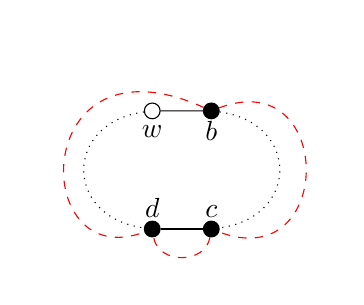
\begin{tikzpicture}[scale=1.5,auto=left,baseline=(d.base)]    
    \begin{scope}[every node/.style={circle,draw=black,fill=white,minimum size=0.2cm, inner sep=0}]
      \node[label=-90:$b$,fill=black] (b) at (0.25,1) {};
      \node[label=-90:$w$] (w) at (-0.25,1) {};
      \node[label=90:$d$,fill=black] (d) at (-0.25,0) {};
      \node[label=90:$c$,fill=black] (c) at (0.25,0) {};
      
      \foreach \from/\to in {b/w,d/c}
	\draw (\from) -- (\to);
	
       \draw[dotted] (b) .. controls (1,0.9) and (1,0.1) .. (c);
       \draw[dotted] (w) .. controls (-1,0.9) and (-1,0.1) .. (d);
       
        \draw[dashed,red] (b) .. controls (1.3,1.4) and (1.3,-0.4) .. (c);
        \draw[dashed,red] (b) .. controls (-1.3,1.7) and (-1.3,-0.4) .. (d);
        \draw[dashed,red] (c) .. controls (0.2,-0.3) and (-0.2,-0.3) .. (d);
%        \draw[dashed,red] (b) .. controls (-1.5,1.8) and (-1,-0.4) .. (0,-0.25);
    \end{scope}
  \end{tikzpicture}
 
  \caption{Illustration of Claim \ref{claim:colourdeg2black}. Dashed lines represent the edges of the blocking graph. Note that we may have $b=c$. Left: $B$, right: $B'$. Since $\block_{B}^+(G)$ is a cycle and $d \notin B$, then $\block_{B'}^+(G)$ is also a cycle with $|B'| = |B| +1$.}
  \label{fig:colourdeg2black}
  
\end{figure}
  
Let $x$ be the neighbour of $b$ on the outside face of $H$ such that $x\not=w$. Such a neighbour exists since $H$ must have at least three vertices. $x$ is white, as otherwise the inner face adjacent to the edge $\{b,x\}$ would have two black vertices, but each inner face has exactly one such vertex by Lemma \ref{lem:blocking_out}. If $x$ is adjacent to a vertex in $V(G)\setminus V(H)$, then there exists a blocking set $B'$ such that $\block_{B'}^+(G)$ is even by Claim \ref{claim:add_blocker_leg}. Thus, we may assume $x$ is not adjacent to any vertex in $V(G)\setminus V(H)$.

Let $F_{\{b,x\}}$ be the inner face of $H$ that is adjacent to the edge $\{b,x\}$. If $x$ is not adjacent to any other internal face than $F_{\{b,x\}}$, it implies that $\deg_G(x)=2$, so there exists a blocking set $B'$ such that $\block_{B'}^+(G)$ is even by Claim \ref{claim:colourdeg2black}. Thus, assume $x$ is adjacent to at least one other internal face. $x$ must be connected via a chord to at least one other vertex of $H$. Let $y$ be the first vertex connected via a chord $c$ to $x$ when doing a walk counterclockwise around $G$ from $x$. $c$ splits $H$ into two subgraphs $H'$ and $H''$, and without loss of generality, $b$ is incident to $H'$ (see Figure \ref{fig:splitH_Hprime}).

\begin{figure}[!ht]
  \centering
  
  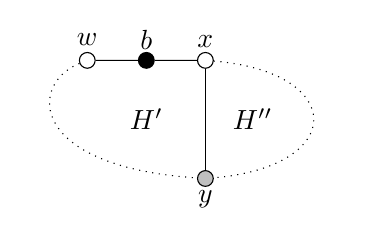
\begin{tikzpicture}[scale=1.5,auto=left,baseline=(y.base)]
    
    \node[] at (-0.5,0.5) {$H'$};
    \node[] at (0.4,0.5) {$H''$};
    
    \begin{scope}[every node/.style={circle,draw=black,fill=white,minimum size=0.2cm, inner sep=0}]
      \node[label=-90:$y$,fill=lightgray] (y) at (0,0) {};
      \node[label=90:$x$] (x) at (0,1) {};
      \node[label=90:$b$,fill=black] (w) at (-0.5,1) {};
      \node[label=90:$w$] (v) at (-1,1) {};
      
      \foreach \from/\to in {x/y,x/w,w/v}
	\draw (\from) -- (\to);
	
       \draw[dotted] (x) .. controls (1.2,0.9) and (1.2,0.1) .. (y);
       \draw[dotted] (v) .. controls (-1.5,0.8) and (-1.5,0.1) .. (y);
%       
      
    \end{scope}
  \end{tikzpicture}
  \hspace{50px}
  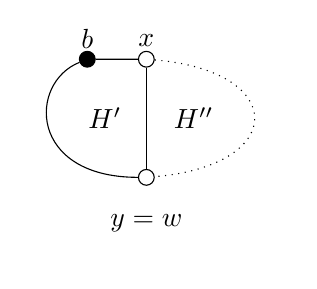
\begin{tikzpicture}[scale=1.5,auto=left,baseline=(y.base)]
    
    \node[] at (-0.35,0.5) {$H'$};
    \node[] at (0.4,0.5) {$H''$};
    
    \begin{scope}[every node/.style={circle,draw=black,fill=white,minimum size=0.2cm, inner sep=0}]
      \node[label=-90:{$y=w$}] (y) at (0,0) {};
      \node[label=90:$x$] (x) at (0,1) {};
      \node[label=90:$b$,fill=black] (w) at (-0.5,1) {};
      
      \foreach \from/\to in {x/y,x/w}
	\draw (\from) -- (\to);
	
       \draw[dotted] (x) .. controls (1.2,0.9) and (1.2,0.1) .. (y);
       \draw (w) .. controls (-1,0.8) and (-1,0) .. (y);
%       
      
    \end{scope}
  \end{tikzpicture}
  \caption{$x$ is adjacent to at least two internal faces. $y$ is the first vertex connected with a chord to $x$ that is found when doing a walk counterclockwise from $x$. We may have $w \not=y$ (left) or $w=y$ (right).}
  \label{fig:splitH_Hprime}
  
\end{figure}
  
Since $H''$ is outerplanar, it contains an ear, which is a face of degree at most 1 in the weak dual. Let $F_e$ be an ear of $H''$ that is incident to a vertex of degree 2 in $H''$ other than $x$ or $y$. Such an ear exists because if $F_e$ is the only face of $H''$, then it is adjacent to at least three vertices, two of them being $x$ and $y$. Otherwise, it must contain an ear that is not adjacent to at most one of $x,y$. This ear is adjacent to at least one vertex of degree 2 that is neither $x$ not $y$. Let the anchors of $F_e$ be the vertices of $F_e$ in $\{z \in V(H'') \;|\; \deg_{H''}(z)\geq 3\} \cup \{x,y\}$. There are exactly two such vertices (Figure \ref{fig:faceAnchorsHprimeprime}). 

\begin{figure}[!ht]
  \centering
  
  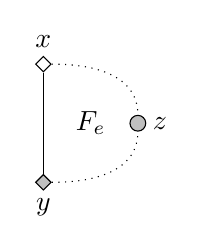
\begin{tikzpicture}[scale=1.5,auto=left,baseline=(y.base)]   
    \begin{scope}[every node/.style={diamond,draw=black,fill=lightgray,minimum size=0.2cm, inner sep=0}]
      \node[label=-90:$y$] (y) at (0,0) {};
      \node[label=90:$x$,fill=white] (x) at (0,1) {};
      \node[circle,label=0:$z$] (d) at (0.8,0.5) {};
      
      \foreach \from/\to in {x/y}
	\draw (\from) -- (\to);
      
      \draw[dotted] (y) .. controls (0.2,0) and (0.8,0) .. (d);
      \draw[dotted] (x) .. controls (0.2,1) and (0.8,1) .. (d);
    \end{scope}
    
    \node[] at (0.4,0.5) {$F_e$};
    
  \end{tikzpicture}
  \hspace{25px}
  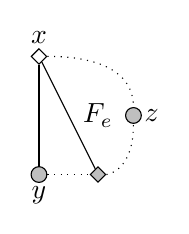
\begin{tikzpicture}[scale=1.5,auto=left,baseline=(y.base)]   
    \begin{scope}[every node/.style={circle,draw=black,fill=lightgray,minimum size=0.2cm, inner sep=0}]
      \node[diamond,label=90:$x$,fill=white] (x) at (0,1) {};
      \node[label=-90:$y$] (y) at (0,0) {};
      \node[diamond] (c) at (0.5,0) {};
      \node[circle,label=0:$z$] (d) at (0.8,0.5) {};
      
      \foreach \from/\to in {x/y,x/c}
	\draw (\from) -- (\to);
	
	\draw[dotted] (y) -- (c);
      
      \draw[dotted] (x) .. controls (0.2,1) and (0.8,1) .. (d);
      \draw[dotted] (c) .. controls (0.55,0) and (0.8,0) .. (d);
    \end{scope}
    
    \node[] at (0.5,0.5) {$F_e$};
    
  \end{tikzpicture}
  \hspace{25px}
  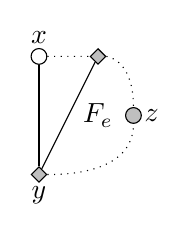
\begin{tikzpicture}[scale=1.5,auto=left,baseline=(y.base)]   
    \begin{scope}[every node/.style={circle,draw=black,fill=lightgray,minimum size=0.2cm, inner sep=0}]
      \node[label=90:$x$,fill=white] (x) at (0,1) {};
      \node[diamond,label=-90:$y$] (y) at (0,0) {};
      \node[diamond] (c) at (0.5,1) {};
      \node[circle,label=0:$z$] (d) at (0.8,0.5) {};
      
      \foreach \from/\to in {x/y,y/c}
	\draw (\from) -- (\to);
	
	\draw[dotted] (x) -- (c);
      
      \draw[dotted] (y) .. controls (0.2,0) and (0.8,0) .. (d);
      \draw[dotted] (c) .. controls (0.55,1) and (0.8,1) .. (d);
    \end{scope}
    
    \node[] at (0.5,0.5) {$F_e$};
    
  \end{tikzpicture}
  \hspace{25px}
  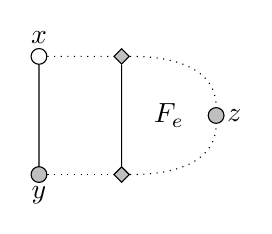
\begin{tikzpicture}[scale=1.5,auto=left,baseline=(y.base)]   
    \begin{scope}[every node/.style={circle,draw=black,fill=lightgray,minimum size=0.2cm, inner sep=0}]
      \node[label=-90:$y$] (y) at (0.3,0) {};
      \node[label=90:$x$,fill=white] (x) at (0.3,1) {};
      \node[diamond] (a) at (1,1) {};
      \node[diamond] (b) at (1,0) {};
      \node[label=0:$z$] (d) at (1.8,0.5) {};
      
      \foreach \from/\to in {x/y,a/b}
	\draw (\from) -- (\to);
	
      \foreach \from/\to in {y/b,x/a}
	\draw[dotted] (\from) -- (\to);
      
      \draw[dotted] (b) .. controls (1.2,0) and (1.8,0) .. (d);
      \draw[dotted] (a) .. controls (1.2,1) and (1.8,1) .. (d);
    \end{scope}
    
    \node[] at (1.4,0.5) {$F_e$};
    
  \end{tikzpicture}
  \caption{Anchors of $F_e$ (anchors represented with diamonds). There are four cases.}
  \label{fig:faceAnchorsHprimeprime}
  
\end{figure}

If one of the anchors is black, then its non-anchor neighbour on $F_e$ has degree 2 on $H$ and is white, therefore there exists a blocking set $B'$ such that $\block_{B'}^+(G)$ is even by Claim \ref{claim:add_blocker_leg} or by Claim \ref{claim:colourdeg2black}. Thus, assume no anchor of $F_e$ is black. Then, one of the non-anchor vertices of $F_e$, say $z$, must be in black. If there is more than one non-anchor vertex on $F_e$, then one of these vertices is adjacent to $z$ and has degree 2 in $H$, and there exists a blocking set $B'$ such that $\block_{B'}^+(G)$ is even by Claim \ref{claim:add_blocker_leg} or by Claim \ref{claim:colourdeg2black}. Thus, assume there is only one non-anchor vertex on $F_e$. We may then assume every ear of $H''$ is a cycle on three vertices with the non-anchor vertex black (Figure \ref{fig:everyEarIsThreeCycle}), as we could otherwise find a vertex for which one of Claim \ref{claim:add_blocker_leg} or Claim \ref{claim:colourdeg2black} could be applied to get a blocking set $B'$ such that $\block_{B'}^+(G)$ is an even cycle.

\begin{figure}[!ht]
  \centering
  
  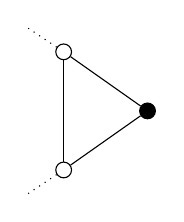
\begin{tikzpicture}[scale=1.5,auto=left]
    
    
    \begin{scope}[every node/.style={circle,draw=black,fill=white,minimum size=0.2cm, inner sep=0}]
      \node[] (a) at (0,0) {};
      \node[] (b) at (0,1) {};
      \node[fill=black] (c) at (0.71,0.5) {};
      
      \foreach \from/\to in {a/b,b/c,c/a}
	\draw (\from) -- (\to);
	
      \draw[dotted] (a) -- (-0.3,-0.2);
      \draw[dotted] (b) -- (-0.3,1.2);
%       
      
    \end{scope}
  \end{tikzpicture}
  \caption{Every ear of $H''$ is a cycle on three vertices with the non-anchor vertex in $B$ and the anchor vertices not in $B$.}
  \label{fig:everyEarIsThreeCycle}
  
\end{figure}

If $H''$ has only one face, then by the choice of $y$, $x$ is adjacent to exactly two inner faces of $H$, one of them adjacent to $b$ and the other is an ear of $H''$ (Figure \ref{fig:ifOneFaceHprimeprime}). Let $z$ be the vertex of degree 2 on $H$ incident to this ear. $z$ is black. Thus, $B'=\{x\} \cup B$ is a blocking set since $\deg_{H\setminus B}(x)=1$, so it is not a cut vertex of $H\setminus B$ and adding it to $B'$ does not disconnect $H\setminus B'$, so we have that $\block_{B'}^+(G)$ is an even cycle. It remains to consider the case where $H''$ has more than one face.

\begin{figure}[!ht]
  \centering
  
  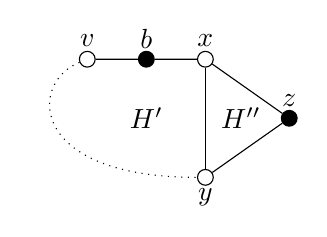
\begin{tikzpicture}[scale=1.5,auto=left,baseline=(y.base)]
    
    \node[] at (-0.5,0.5) {$H'$};
    \node[] at (0.3,0.5) {$H''$};
    
    \begin{scope}[every node/.style={circle,draw=black,fill=white,minimum size=0.2cm, inner sep=0}]
      \node[label=-90:$y$] (y) at (0,0) {};
      \node[label=90:$x$] (x) at (0,1) {};
      \node[label=90:$b$,fill=black] (w) at (-0.5,1) {};
      \node[label=90:$v$] (v) at (-1,1) {};
      \node[label=90:$z$,fill=black] (z) at (0.71,0.5) {};
      
      \foreach \from/\to in {x/y,x/w,w/v,x/z,y/z}
	\draw (\from) -- (\to);
	
       \draw[dotted] (v) .. controls (-1.5,0.8) and (-1.5,0) .. (y);
      
    \end{scope}
  \end{tikzpicture}
  \hspace{50px}
  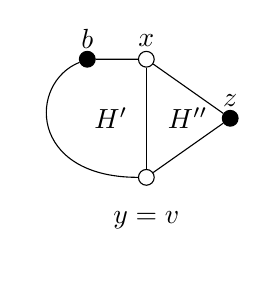
\begin{tikzpicture}[scale=1.5,auto=left,baseline=(y.base)]
    
    \node[] at (-0.3,0.5) {$H'$};
    \node[] at (0.35,0.5) {$H''$};
    
    \begin{scope}[every node/.style={circle,draw=black,fill=white,minimum size=0.2cm, inner sep=0}]
      \node[label=-90:{$y=v$}] (y) at (0,0) {};
      \node[label=90:$x$] (x) at (0,1) {};
      \node[label=90:$b$,fill=black] (w) at (-0.5,1) {};
      \node[label=90:$z$,fill=black] (z) at (0.71,0.5) {};
      
      \foreach \from/\to in {x/y,x/w,x/z,y/z}
	\draw (\from) -- (\to);
	
       \draw (w) .. controls (-1,0.8) and (-1,0) .. (y);
%       
      
    \end{scope}
  \end{tikzpicture}
  \caption{$H''$ has only one face. We constructed $H''$ such that all chords from $x$ are in $H''$, thus $x$ only has one chord, $\{x,y\}$. We can have $v\not=y$ (left) or $v=y$ (right).}
  \label{fig:ifOneFaceHprimeprime}
  
\end{figure}
%\FloatBarrier
Let $F$ be a face of $H'$ that is adjacent to the edge $\{x,y\}$. Let $T$ be the weak dual of $H'' \cup F$. $T$ is a tree since $H'' \cup F$ is outerplanar. Root $T$ at $F$ and do a breadth-first search on $T$. The height\footnote{The \emph{height} of a tree is the eccentricity of its root.} $h$ of $T$ must be at least 2 since $F$ has degree 1 in $T$ and $H''$ has at least two faces, only one of which is adjacent to $F$. Let $F^{\dagger}$ be a face of $T$ that has depth $h-1$ in $T$ (it is on the second layer from the bottom in the breadth-first search layering of $T$). All the children of $F^{\dagger}$ in $T$ are leaves, thus they must be ears of $H''$. Let $\{l,k\}$ be the edge that divides $F^{\dagger}$ and its parent in $T$. Without loss of generality, let $k$ be white (they cannot both be black). %Note that we may have $l=y$ or $k=x$. 

\begin{figure}[!ht]
  \centering
  
  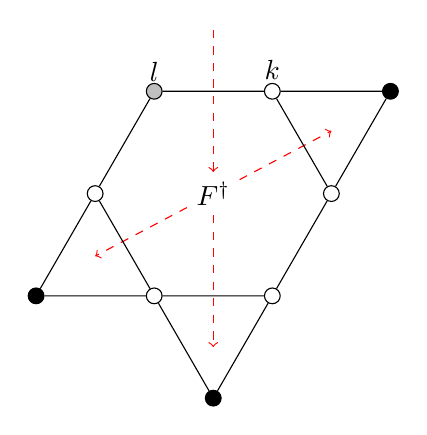
\begin{tikzpicture}[scale=1.5,auto=left]
    
     \node[] (fstar) at (0,0) {$F^{\dagger}$};
     
     \draw[dashed,red,<-] (fstar) -- (0,1.4);
     \draw[dashed,red,->] (fstar) -- (-1,-0.53);
     \draw[dashed,red,->] (fstar) -- (1,0.53);
     \draw[dashed,red,->] (fstar) -- (0,-1.3);
%     \node[] at (0.3,0.5) {$H''$};
    
    \begin{scope}[every node/.style={circle,draw=black,fill=lightgray,minimum size=0.2cm, inner sep=0}]
      \node[label=90:$l$] (l) at (-0.5,0.866) {};
      \node[label=90:$k$,fill=white] (k) at (0.5,0.866) {};
      \node[fill=white] (a) at (-1,0) {};
      \node[fill=white] (b) at (1,0) {};
      \node[fill=white] (c) at (-0.5,-0.866) {};
      \node[fill=white] (d) at (0.5,-0.866) {};
      
      \node[fill=black] (e) at (-1.5,-0.866) {};
      \node[fill=black] (f) at (0,-1.732) {};
      \node[fill=black] (g) at (1.5,0.866) {};
      
      \foreach \from/\to in {l/k,k/b,b/d,d/c,c/a,a/l,a/e,e/c,c/f,d/f,b/g,k/g}
	\draw (\from) -- (\to);
	
%        \draw[dotted] (v) .. controls (-1.5,0.8) and (-1.5,0) .. (y);
      
    \end{scope}
  \end{tikzpicture}
  \caption{A possible configuration for $F^{\dagger}$ and its children. In dashed: the weak dual corresponding to these faces, with arrows pointing away from $F$.}
  \label{fig:fStarInHprimeprime}
  
\end{figure}

\begin{figure}[!ht]
  \centering
  
  \begin{subfigure}[t]{0.3\textwidth}
    \centering
    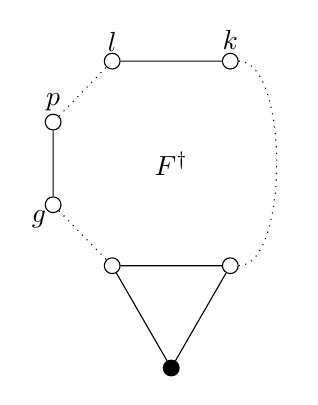
\begin{tikzpicture}[scale=1.5,auto=left]
      
      \node[] (fstar) at (0,0) {$F^{\dagger}$};
      
      \begin{scope}[every node/.style={circle,draw=black,fill=white,minimum size=0.2cm, inner sep=0}]
	\node[label=90:$l$] (l) at (-0.5,0.866) {};
	\node[label=90:$k$] (k) at (0.5,0.866) {};
	\node[label=90:$p$] (p) at (-1,0.35) {};
	\node[label=-135:$g$] (g) at (-1,-0.35) {};
	%\node[fill=pink] (b) at (1,0) {};
	\node[] (c) at (-0.5,-0.866) {};
	\node[] (d) at (0.5,-0.866) {};
	
	\node[fill=black] (f) at (0,-1.732) {};
	%\node[fill=black] (g) at (1.5,0.866) {};
	
	\foreach \from/\to in {l/k,d/c,g/p,c/f,d/f}
	  \draw (\from) -- (\to);
	  
	\draw[dotted] (g) -- (c);
	\draw[dotted] (p) -- (l);
	  
	\draw[dotted] (k) .. controls (1,0.866) and (1,-0.866) .. (d);
	
      \end{scope}
    \end{tikzpicture}
    \caption{if $\deg_H(g)=2$, then we use Claim \ref{claim:add_blocker_leg} or Claim \ref{claim:colourdeg2black}.}
    \label{fig:fStar_noDeg2g}
   
  \end{subfigure}
  ~
  \begin{subfigure}[t]{0.3\textwidth}
    \centering
    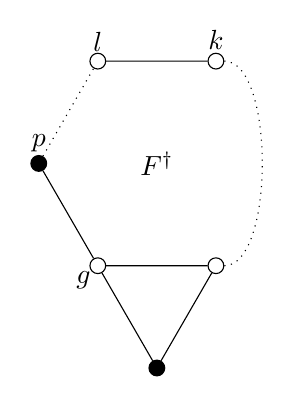
\begin{tikzpicture}[scale=1.5,auto=left]
      
      \node[] (fstar) at (0,0) {$F^{\dagger}$};
      
      \begin{scope}[every node/.style={circle,draw=black,fill=white,minimum size=0.2cm, inner sep=0}]
	\node[label=90:$l$] (l) at (-0.5,0.866) {};
	\node[label=90:$k$] (k) at (0.5,0.866) {};
	\node[label=90:$p$,fill=black] (a) at (-1,0) {};
	%\node[fill=pink] (b) at (1,0) {};
	\node[label=-135:$g$] (c) at (-0.5,-0.866) {};
	\node[] (d) at (0.5,-0.866) {};
	
	\node[fill=black] (f) at (0,-1.732) {};
	%\node[fill=black] (g) at (1.5,0.866) {};
	
	\foreach \from/\to in {l/k,d/c,a/c,c/f,d/f}
	  \draw (\from) -- (\to);
	  
	\draw[dotted] (k) .. controls (1,0.866) and (1,-0.866) .. (d);
	\draw[dotted] (a) -- (l);
	
      \end{scope}
    \end{tikzpicture}
    \caption{$p\not=l$}
    \label{fig:fStar_pIsNotL}
   
  \end{subfigure}
  ~
  \begin{subfigure}[t]{0.3\textwidth}
    \centering
    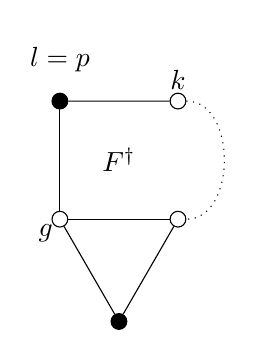
\begin{tikzpicture}[scale=1.5,auto=left]
      
      \node[] (fstar) at (0,0.5) {$F^{\dagger}$};
      
      \begin{scope}[every node/.style={circle,draw=black,fill=white,minimum size=0.2cm, inner sep=0}]
	\node[label=90:{$l=p$},fill=black] (l) at (-0.5,1) {};
	\node[label=90:$k$] (k) at (0.5,1) {};
	%\node[fill=pink] (b) at (1,0) {};
	\node[label=-135:$g$] (c) at (-0.5,0) {};
	\node[] (d) at (0.5,0) {};
	
	\node[fill=black] (f) at (0,-0.866) {};
	%\node[fill=black] (g) at (1.5,0.866) {};
	
	\foreach \from/\to in {l/k,d/c,c/l,c/f,d/f}
	  \draw (\from) -- (\to);
	  
	\draw[dotted] (k) .. controls (1,1) and (1,0) .. (d);
	
      \end{scope}
    \end{tikzpicture}
    \caption{$p=l$}
    \label{fig:fStar_pIsL}
   
  \end{subfigure}
  
  \caption{$p$ and $g$ on $F^{\dagger}$. $F^{\dagger}$ must be adjacent to at least one ear of $H''$ by choice of $F^{\dagger}$.}
  \label{fig:pgOnFstar}
  
\end{figure}

Let $p$ be the black vertex incident to $F^{\dagger}$. If $p$ is incident to a child of $F'$, or if any child of $F^{\dagger}$ has more than three vertices, then we can apply one of the previous arguments.
Let $g$ be the neighbour of $p$ along $F^{\dagger}$ other than $l$ or $k$. Such a vertex must exist otherwise there would be two black vertices on an ear of $F^{\dagger}$. Then, the edge $\{p,g\}$ is adjacent to the outside face since $p$ cannot be incident to any children of $F^{\dagger}$. We may assume that $g$ is not adjacent to any vertex in $V(G)\setminus V(H)$ and that  $\deg_G(g)\not=2$, since otherwise there exists a blocking set $B'$ such that $\block_{B'}^+(G)$ is even by Claim \ref{claim:add_blocker_leg} or by Claim \ref{claim:colourdeg2black} (Figure \ref{fig:fStar_noDeg2g}). Thus, we may assume that $\deg_G(g)\geq 3$ and is not adjacent to a vertex in  $V(G)\setminus V(H)$. Then, $F^{\dagger}$ has the configuration of Figure \ref{fig:fStar_pIsNotL} or Figure \ref{fig:fStar_pIsL}. 

Note that since $g \in V(H'') \setminus \{l,k\}$, this implies that $g \not= w$. Thus, $B' = \{g\} \cup B$ is a blocking set as $\deg_{H\setminus B}(g)=1$, so $g$ is not a cut vertex of $H\setminus B$, and adding it to $B'$ does not disconnect $H\setminus B'$, and we have that $|\block_{B'}^+(G)|$ is even. This completes the proof. 
\end{proof}
The following lemma shows how to use Lemma \ref{lem:cycle_spider_even} to create a blocking graph of any outerplane graph such that every cycle of the blocking graph is even.

\begin{lemma}
 There exists a blocking set $B$ of $G$ such that every cycle in $\block_{B}(G)$ is even.
 \label{lem:exists_even_blocking_graph}
\end{lemma}

\begin{proof}
 Assume that $G$ is not a tree since in this case, an empty blocking set satisfies the condition. Also, assume that $G$ is connected, otherwise we may apply the lemma for each of its connected components. Let $S_1,S_2,\ldots,S_k$ be subgraphs of $G$ such that: 1) each $S_i$ is a spider graph and 2) for each $i \in \{2,\ldots,k\}$, if $H_i$ is the 2-connected component of $S_i$, then
\begin{enumerate}[a)]
 \item $V(S_i) \cap V(S_{i-1}) = \{v\}$ such that $v \in V(H_i)$,
 \item $S_{i-1} \setminus S_i$ is connected,
 \item $V(G)= V(S_1) \cup V(S_2) \cup \cdots \cup V(S_k)$ and
 \item $E(G)= E(S_1) \cup E(S_2) \cup \cdots \cup E(S_k)$
\end{enumerate} 
 (see Figure \ref{fig:all_cycles_even}). Let $B_1$ be a blocking set of $S_1$ such that $\block_{B_1}^+(S_1)$ is an even cycle. Such a set exists by Lemma \ref{lem:cycle_spider_even}. For each spider graph $S_i$ for $i \in \{2,\ldots,k\}$, let $v$ be the vertex $v \in V(S_i) \cap V(S_{i-1})$. Let $u$ be a neighbour of $v$ on $H_i$. If $v \in B_{i-1}$, there exists a blocking set $B_i$ of $S_i$ in which $v \in B_i$ and $u \notin B_i$ by Lemma \ref{lem:cycle_spider_even}. Similarly, if $v \notin B_{i-1}$, there exists a blocking set $B_i$ in which $v \notin B_i$ and $u \in B_i$. In both cases, $\block_{B_i}^+(S_i)$ is an even cycle.
 
 Let $B = \bigcup_{1 \leq i \leq k} B_i$. Observe that $B$ is a blocking set of $G$. For each cycle $C$ of $\block_{B}^+(G)$, if $V(C) \subseteq V(S_i)$ for some $S_i$, then $C$ is even. Otherwise, $C$ includes vertices in multiple spider graphs $S'_1,\ldots,S'_l$ with blocking sets $B'_1,\ldots,B'_l$. Let $\mathcal{S}_C = \{S'_1,\ldots,S'_l\}$. Notice that
 \begin{equation}
  \bigcup_{1 \leq j_1 < j_2 \leq l} (B'_{j_1} \cap B'_{j_2}) = \emptyset,
 \end{equation}
 otherwise $\block_{B}^+(\mathcal{S}_C)$ would contain at least two simple cycles. Thus, 
 \begin{equation}
 \left|V(\block_{B}^+(\mathcal{S}_C))\right|= \sum_{1 \leq j \leq l} |V(\block_{B}^+(S'_j))|
 \end{equation}
 and since each of $|V(\block_{B}^+(S'_j))|$ is even, $|V(\block_{B}^+(\mathcal{S}_C))|$ is also even. Therefore, all cycles of $\block_{B}^+(G)$ are even, which implies that all cycles of $\block_{B}(G)$ are also even since $E(\block_{B}(G)) \subseteq E(\block_{B}^+(G))$. This completes the proof.
\end{proof}

\begin{figure}[!ht]
  \centering
  
  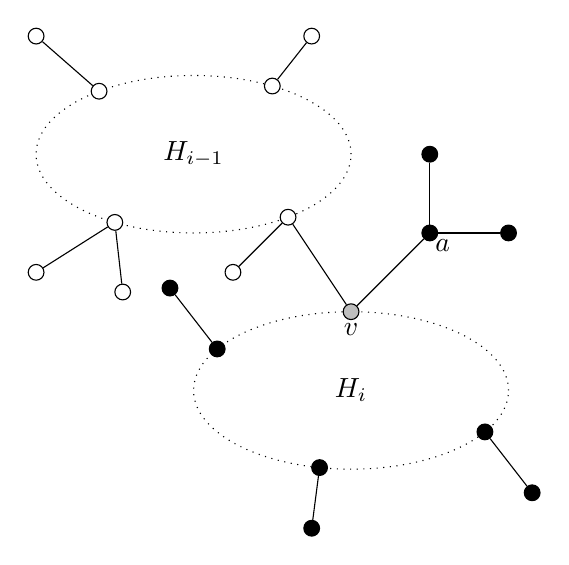
\begin{tikzpicture}[scale=1,auto=left]
    
    \node at (0,0) {$H_{i-1}$};
    \node at (2,-3) {$H_{i}$};
    
    \begin{scope}[every node/.style={circle,draw=black,fill=white,minimum size=0.2cm, inner sep=0}]
% 	\draw[step=1cm,lightgray,very thin] (-2,-2) grid (2,2);
	\draw[dotted] (0,0) ellipse (2cm and 1cm);
	
	\node (a1) at (1,0.866) {};
	\node (a2) at (-1.2,0.8) {};
	\node (u) at (1.2,-0.8) {};
	\node (a3) at (-1,-0.866) {};
	
	\node (b1) at (1.5,1.5) {};
	\node (b2) at (-2,1.5) {};
 	\node (b3) at (-0.9,-1.75) {};
 	\node (b3b) at (-2,-1.5) {};
	\node (b4) at (0.5,-1.5) {};
    
%       \node[label=90:$l$] (l) at (-0.5,0.866) {};
      
      \foreach \from/\to in {a1/b1,a2/b2,a3/b3,a3/b3b,u/b4}
	\draw (\from) -- (\to);

      
    \end{scope}
    
    \begin{scope}[shift={(2,-3)},every node/.style={circle,draw=black,fill=black,minimum size=0.2cm, inner sep=0}]
% 	\draw[step=1cm,lightgray,very thin] (-2,-2) grid (2,2);
	\draw[dotted] (0,0) ellipse (2cm and 1cm);
	
	\node[fill=lightgray,label=-90:$v$] (v) at (0,1) {};
	\node (c1) at (-1.7,0.5268) {};
	\node (c2) at (1.7,-0.5268) {};
	\node (c3) at (-0.4,-0.9798) {};
	
	\node (d1) at (-2.3,1.3) {};
	\node (d2) at (2.3,-1.3) {};
	\node (d3) at (-0.5,-1.75) {};
	\node[label=-45:$a$] (d4) at (1,2) {};
	\node (d4b) at (1,3) {};
	\node (d4c) at (2,2) {};
    
%       \node[label=90:$l$] (l) at (-0.5,0.866) {};
      
       \foreach \from/\to in {c1/d1,c2/d2,c3/d3,v/d4,u/v,d4/d4b,d4/d4c}
 	\draw (\from) -- (\to);
      
    \end{scope}
  \end{tikzpicture}
  \caption{Two spider graphs $S_{i-1}, S_i$ of some outerplane graph. Vertices in white are part of $S_{i-1}$, vertices in black are part of $S_i$, and $v$, in gray, is part of both. Notice that $a$ must be part of $S_i$, otherwise $S_{i-1}\setminus{S_i}$ would not be connected.}
  \label{fig:all_cycles_even}
  
\end{figure}

\subsection{Main Results}

We are now ready to prove the main results for this section.

\begin{theorem}
 \thmfacialoutplanar
\label{thm:facial_outplanar}
\end{theorem}

\begin{proof}
Let $B$ be a blocking set of $G$ such that every cycle in $\block_{B}(G)$ is even. Such a set exists by Lemma \ref{lem:exists_even_blocking_graph}. By Lemma \ref{lem:outer_face_cactus}, there exists a facial nonrepetitive 7-colouring of $\block_{B}(G)$. Thus, by Lemma \ref{lem:hitting_plus_four}, there exists a facial nonrepetitive 11-colouring of $G$. This completes the proof. 
\end{proof}

As mentioned earlier, we can improve this bound for outerplane graphs that contain at most one 2-connected component.

\begin{theorem}
 \thmfacialoutplanarbic
\label{thm:facial_outplanar_bic}
\end{theorem}
We will need the following claim:

\begin{claim}
 Let $G$ be a 2-connected outerplane graph. There exists a blocking set $B$ of $G$ such that 
 $|B| \notin \{5, 7, 9, 10, 14, 17\}.$
 \label{claim:existsNoBadBlocking}
\end{claim}

\begin{proof}
 If $G$ is a cycle, then any set that contains one vertex of $G$ respects this constraint. Thus, assume $G$ has at least two inner faces.
 By Corollary \ref{cor:blocking_out_select}, there exists a blocking set $B$ of $G$ such that $F_1$ is a face of degree 1 in $\wdual{G}$ and $v \in B\cap V(F_1)$ such that $\deg_G(v) \geq 3$. 
 If $|B| \notin \{5, 7, 9, 10, 14, 17\}$, then we are done. Thus, suppose $|B| \in \{5, 7, 9, 10, 14, 17\}$. There must be at least 5 inner faces in $G$, as there is at most one vertex in $B$ for each inner face of $G$.
 Since $v \in V(F_1) \cap B$ has degree at least three and $F_1$ has degree 1 in  $\wdual{G}$, there must be a vertex $u \in V(F_1) \setminus B$ such that $\deg_G(u) =2$ and $\{u,v\}\in E(G)$ (Figure \ref{fig:addfirst}). Thus, $u$ is not a cut vertex of $G \setminus B$ which implies that $B' = \{u \} \cup B$ is a blocking set of $G$. Furthermore, $|B'|=|B+1|$, so if $|B| \in \{5, 7, 10, 14, 17\}$, then $|B'| \notin \{5, 7, 9, 10, 14, 17\}$ and we are done. Therefore, assume $|B|=9$, thus $|B'|=10$. 
 
  \begin{figure}[!ht]
  \centering
  
  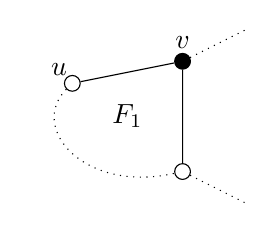
\begin{tikzpicture}[scale=1.4,auto=left]
    
    \node at (0.5,0.5) {$F_1$};
    
    \begin{scope}[every node/.style={circle,draw=black,fill=white,minimum size=0.2cm, inner sep=0}]
      \node[label=$v$,fill=black] (n) at (1,1) {};
      \node[] (a) at (1,0) {};
      \node[label=135:$u$] (z) at (0,0.8) {};
      % left, up
      \foreach \from/\to in {z/n,n/a}
	\draw (\from) -- (\to);
	
      \draw[dotted] (z) .. controls (-0.4,0.4) and (0.1,-0.2) .. (a);
      
      \draw[dotted] (n) -- (1.6,1.3);
      \draw[dotted] (a) -- (1.6,-0.3);
      
    \end{scope}
  \end{tikzpicture}

  \caption{$B'=\{u\} \cup B$ is a blocking set of $G$.}
  \label{fig:addfirst}  
\end{figure}
 
 We will now show how to add another vertex to the blocking set. Let us again say that a vertex $u\in V(G)$ is \emph{black} if $u \in B'$ and is \emph{white} otherwise. If there exists an edge $\{b,w\}\in E(G)$ that is incident to the outer face and such that $b$ is black, $w$ is white and $\deg_G(w)=2$, let $B''=\{w\} \cup B'$. We must have $\deg_{G \setminus B'}(w)=1$, so $w$ is not a cut vertex of $G \setminus B'$, so $B''$ is a blocking set of $G$ with $|B''|=|B'|+1$, thus $|B''|=11 \notin \{5, 7, 9, 10, 14, 17\}$ and we are done. Thus, we may assume that no such edge exists. 
 
 $\wdual{G}$ is a tree since $G$ is outerplanar. Root $\wdual{G}$ at $F_1$ and do a breadth-first search on $\wdual{G}$. The height $h$ of $\wdual{G}$ must be at least 3 since $G$ is 2-connected and contains at least five faces. Let $F$ be a face of $\wdual{G}$ that has height $h-1$ in $\wdual{G}$ (thus it is on the second layer from the bottom in the breadth-first search layering of $\wdual{G}$). All the children of $F$ in $\wdual{G}$ are leaves, and none of them are $F_1$. Let $x$ be the black vertex incident to $F$. Note that $x$ cannot be incident to any child of $F$ in $\wdual{G}$, as in this case we could find a $\{b,w\}$ edge on this child, but that is a contradiction. For the same reason, no neighbour of $x$ incident to $F$ can have degree 2, so all neighbours of $x$ must have degree at least 3. Also, by choice of $F$, at least one such neighbour, say $y$, must be incident to exactly two faces: $F$ and some face $F'$ that is a child of $F$ in $\wdual{G}$. Let $z$ be the black vertex on $F'$. By our reasoning, $z$ must be adjacent to $y$ (see Figure \ref{fig:addsecond_2}). Let $B''=\{y\} \cup B'$. Since $\deg_{G \setminus B'}(y)=1$, $u$ is not a cut vertex of $G \setminus B'$, so $B''$ is a blocking set of $G$ with $|B''|=|B'|+1$, thus $|B''|=11 \notin \{5, 7, 9, 10, 14, 17\}$ and we are done. 
\end{proof}
 
 \begin{figure}[!ht]
  \centering
  
  \begin{tikzpicture}[scale=1.2,auto=left]
    
    \node at (2,1.3) {$F'$};
    \node at (1.5,0.5) {$F$};
    
    \begin{scope}[every node/.style={circle,draw=black,fill=white,minimum size=0.2cm, inner sep=0}]
      \node[label=$x$,fill=black] (x) at (0,1) {};
      \node[label=$y$] (b) at (1,1) {};
      \node[] (c) at (3,1) {};
      \node[label=$z$,fill=black] (a) at (2,2) {};
      % left, up
      \foreach \from/\to in {x/b,b/c,b/a,c/a}
	\draw (\from) -- (\to);
	
      \draw[dotted] (x) .. controls (-1,-0.5) and (4.5,-0.5) .. (c);
      
    \end{scope}
  \end{tikzpicture}
  ~
  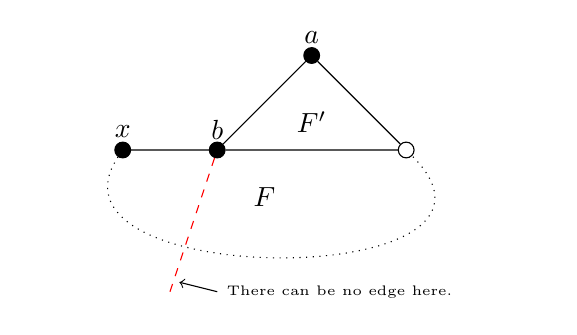
\begin{tikzpicture}[scale=1.2,auto=left]
    
    \node at (2,1.3) {$F'$};
    \node at (1.5,0.5) {$F$};
    
    \begin{scope}[every node/.style={circle,draw=black,fill=white,minimum size=0.2cm, inner sep=0}]
      \node[label=$x$,fill=black] (x) at (0,1) {};
      \node[label=$b$, fill=black] (b) at (1,1) {};
      \node[] (c) at (3,1) {};
      \node[label=$a$,fill=black] (a) at (2,2) {};
      % left, up
      \foreach \from/\to in {x/b,b/c,b/a,c/a}
	\draw (\from) -- (\to);
	
      \draw[dotted] (x) .. controls (-1,-0.5) and (4.5,-0.5) .. (c);
      
      \draw[dashed,red] (b) -- (0.5,-0.5);
      
    \end{scope}
    
    \draw[->] (1,-0.5) -- (0.6,-0.4);
    \node[font=\tiny,anchor=west] at (1,-0.5) {There can be no edge here.};
    
    
  \end{tikzpicture}
  
  \caption{$B''=\{y\} \cup B'$ is a blocking set of $G$.}
  \label{fig:addsecond_2}
  
  \end{figure}

\begin{proof}[Proof of Theorem \ref{thm:facial_outplanar_bic}]
If $G$ does not contain a 2-connected component, then it is a tree and has a nonrepetitive 4-colouring. Thus, suppose $G$ contains exactly one 2-connected component $H$. By Claim \ref{claim:existsNoBadBlocking}, there exists a blocking set $B$ of $H$ such that $|B| \notin \{5, 7, 9, 10, 14, 17\}$. Note that $B$ is also a blocking set of $G$. If $\block_B(G)$ is a cycle, then there exists a nonrepetitive 3-colouring of $\block_B(G)$ by Theorem \ref{thm:colouring_cycles}. Otherwise, it is a forest of paths, for which a nonrepetitive 3-colouring also exists. Thus, by Lemma \ref{lem:hitting_plus_four}, there exists a facial nonrepetitive 7-colouring of $G$. This completes the proof.  
\end{proof}


\section{Plane Graphs}
\label{sec:facial_plane}

We are now ready to apply Theorem \ref{thm:facial_outplanar} to plane graphs. For this, we use a modified version of Bar{\'a}t and Czap's proof for the facial Thue chromatic number of plane graphs \cite{barat2013facial}. Recall that their proof partitions a plane graph in layers, each of which is an outerplanar graph, which can then be nonrepetitively 12-coloured. By using two 12-colour sets, one for odd-numbered layers and another to even-numbered layers, they are able to show that this construction avoids repetitive paths (see Figure \ref{fig:planar_decomposition}). However, we may not use Theorem \ref{thm:facial_outplanar} directly with their proof to tighten the upper bound, as it requires a nonrepetitive colouring of an outerplanar graph, not a \emph{facial} nonrepetitive colouring of an \emph{outerplane} graph. In the following proof, we show that their approach still works when using these restrictions, that is; each layer is not only an outerplanar graph but is also an outerplane graph, and using a facial nonrepetitive colouring of each layer, again using two colour sets for odd and even numbered layers, is enough to prevent repetitions on facial paths.

\begin{figure}  
  \centering
  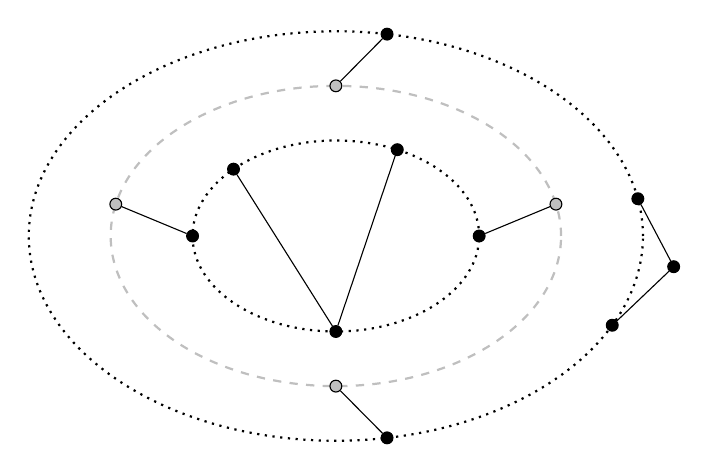
\begin{tikzpicture}[scale=1.3]
            
    \draw[dotted,black,thick] (0,0) ellipse (3cm and 2cm);
    \draw[dashed,lightgray,thick] (0,0) ellipse (2.2cm and 1.4667cm);
    \draw[dotted,black,thick] (0,0) ellipse (1.4cm and 0.933cm);
    
    \begin{scope}[every node/.style={circle,draw=black,fill=white,minimum size=0.15cm, inner sep=0}]

     \node[fill=lightgray] (a) at (0,1.4667) {}; 
     \node[fill=black] (b) at (0.5,1.972) {};
     
     \node[fill=lightgray] (c) at (0,-1.4667) {}; 
     \node[fill=black] (d) at (0.5,-1.972) {};
     
     \node[fill=black] (e) at (1.4,0) {};	
     \node[fill=lightgray] (f) at (2.15,0.311) {};
     
     \node[fill=black] (g) at (-1.4,0) {};	
     \node[fill=lightgray] (h) at (-2.15,0.311) {};
     
     \node[fill=black] (i) at (2.95,0.364) {};
     \node[fill=black] (j) at (2.7,-0.872) {};
     \node[fill=black] (n) at (3.3,-0.3) {};
     
     \node[fill=black] (k) at (0,-0.933) {};
     \node[fill=black] (l) at (0.6,0.843) {};
     \node[fill=black] (m) at (-1,0.653) {};
	 
       \foreach \from/\to in {a/b,c/d,e/f,g/h,i/n,j/n,k/l,k/m}
 	\draw (\from) -- (\to); 
      
    \end{scope}
    
  \end{tikzpicture}
  
  \caption{Visualization of the decomposition of a plane graph into outerplane layers. Each dotted/dashed ellipse corresponds to a layer of vertices, forming an outerplane graph. Dotted layers denoted get coloured with one colour set and vertices on the dashed layer get coloured with a second colour set.}
  \label{fig:planar_decomposition}
  
  \end{figure}

Let $H$ be a plane graph. We define $\delta(H)$ to be the set of vertices in $H$ adjacent to the outer face, and $[\delta(H)]$ to be the subgraph of $H$ induced by $\delta(H)$.

\begin{theorem}
 \thmfacialplanar
 \label{thm:facial_planar_2r}
\end{theorem}


\begin{proof}
 First, we label the vertices of $G$ black or white as follows:
 \begin{enumerate}[a)]
  \item Let $G_1=G$ and $i=1$
  \item While $G_i \not= [\delta(G_i)]$, let $G_{i+1}= G_i \setminus \delta(G_i)$ and $i \gets i+1$
  \item Label every $u \in \delta(G_i)$ black if $i$ is odd or white if $i$ is even.
 \end{enumerate}
 Notice that $[\delta(G_i)]$ is outerplane for every $i$. Let $F$ be a face of $G$. $B(F)$ and $W(F)$ are the set of vertices adjacent to $F$ that are respectively labelled black and white. 
 We create an augmented graph $G^+$ as follows: for each facial path $a,v_1,v_2,\ldots,v_k,b$ such that 
 
%  Let $G^+$ be the graph $G$ with extra edges added: we add an edge $(a,b) \in V(G)\times V(G)$ if and only if 
%  $P=a,v_1,v_2,\ldots,v_k,b$ is a facial path of $G$ such that:
 \begin{enumerate}[a)]
  \item $\{a,b\}\notin E(G)$,
  \item $a,b \in \delta(G_i)$ for some $i$, and
  \item $v_1,v_2,\ldots,v_k \in \delta(G_{i+1})$,
 \end{enumerate} 
 add an edge $\{a,b\}$ to $G^+$ with its curve following the edges of $P$. We denote such $\{a,b\}$ edges as \emph{correction edges}.
 
 \begin{figure}[!ht]
  \centering
  
  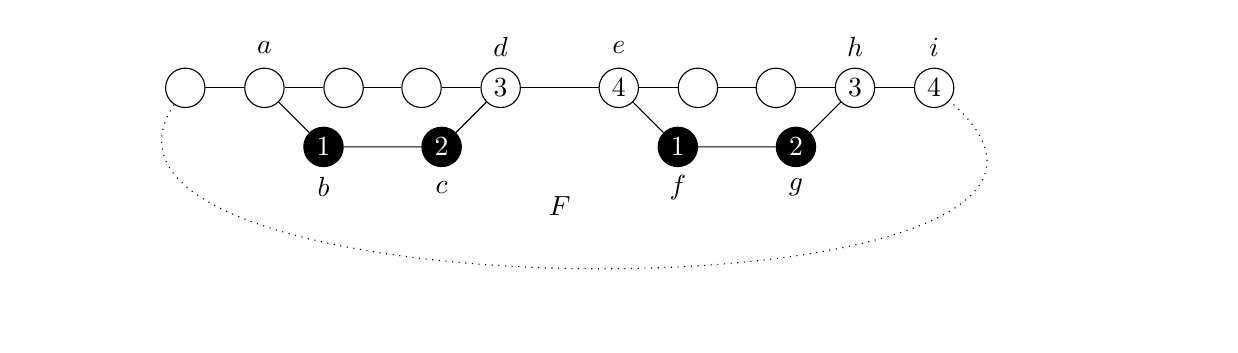
\begin{tikzpicture}[scale=1.5,auto=left]
    
    \node at (-0.5,-1) {$F$};
    
    \begin{scope}[every node/.style={circle,draw=black,minimum size=0.5cm, inner sep=0}]
      \node[label=90:{$e$}] (a1) at (0,0) {$4$};
      \node[fill=none] (b1) at (0.67,0) {};
      \node[fill=none] (c1) at (1.33,0) {};
      \node[label=90:{$h$}] (d1) at (2,0) {$3$};
      \node[label=90:{$i$}] (g1) at (2.67,0) {$4$};
      \node[fill=black,text=white,label=-90:{$f$}] (e1) at (0.5,-0.5) {$1$};
      \node[fill=black,text=white,label=-90:{$g$}] (f1) at (1.5,-0.5) {$2$};
      \node[label=90:{$d$}] (a2) at (-1,0) {$3$};
      \node[fill=none] (b2) at (-1.67,0) {};
      \node[fill=none] (c2) at (-2.33,0) {};
      \node[fill=none,label=90:{$a$}] (d2) at (-3,0) {};
      \node[fill=black,text=white,label=-90:{$c$}] (e2) at (-1.5,-0.5) {$2$};
      \node[fill=black,text=white,label=-90:{$b$}] (f2) at (-2.5,-0.5) {$1$};
      \node[fill=none] (g2) at (-3.67,0) {};
      % left, up
      \foreach \from/\to in {a1/b1,b1/c1,c1/d1,d1/g1,a1/e1,e1/f1,f1/d1,a2/b2,b2/c2,c2/d2,a2/e2,e2/f2,f2/d2,a1/a2,g2/d2}
	\draw (\from) -- (\to);
	
      \draw[dotted] (g2) .. controls (-5,-2) and (5,-2) .. (g1);
      
    \end{scope}
  \end{tikzpicture}
  
  \caption{Correction edges are necessary to prevent repetitions. In this example, the white vertices are part of $\delta(G_i)$ and the black vertices are part of $\delta(G_i+1)$. Labels inside the vertices represent colours. This colouring induces a repetitive path $b,c,d,e,f,g,h,i$. This repetition would be avoided in our construction since there would be a correction edge $\{e,h\}$ in $[\delta(G_i)]^+$, which would prevent the sequence of vertices $d,e,h,i$ to be repetitive.}
  \label{fig:correction_edges}
  
  \end{figure}
 
 Let $[\delta(G_i)]^+$ be the subgraph of $G^+$ induced by $\delta(G_i)$. Notice that each $[\delta(G_i)]^+$ is outerplane as all of its vertices lay on the outside face by construction, and correction edges were added on top of edges of $G$, which was plane, and such edges are not included in $[\delta(G_i)]^+$.
 Let $c_i$ be a facial nonrepetitive $r$-colouring of $[\delta(G_i)]^+$ on colours $\{1,\ldots,r\}$ if $i$ is odd, and colours $\{r+1,\ldots,2r\}$ is $i$ is even. Such a colouring exists by our hypothesis. The union of all these colourings induce a $2r$-colouring $c$ of $G$. We will now show that $c$ is a facial nonrepetitive colouring.
 Suppose that this is not the case. Thus, there exists a facial path $P$ on some face $F$ such that the colour sequence $S$ of vertices in $P$ is repetitive. There are two cases:
 \begin{enumerate}
  \item $P$ is composed of vertices of one of $B(F)$ or $W(F)$ (thus we have $P \setminus{B(F)} = P$ or $P \setminus{W(F)} = P$). Notice that $P$ must be contained in exactly one subgraph of $G$, say $[\delta(G_i)]$. If $P$ is also a facial path of $[\delta(G_i)]^+$, then $P$ cannot be repetitive. Thus, $P$ must not be a facial path in $[\delta(G_i)]^+$. However, the only edges in $[\delta(G_i)]^+$ that are not in $[\delta(G_i)]$ are correction edges, which are located on top of paths in $G$. Therefore, the vertices of $P$ must not be consecutive on a single face, which is a contradiction.
  
  \item $P$ is composed of vertices of both $B(F)$ and $W(F)$. It must lay on exactly two subgraphs of $G$, say $[\delta(G_i)]$ and $[\delta(G_{i+1})]$, as otherwise it would not be a facial path. Since the colours classes of vertices in $\delta(G_i)$ and of vertices in $\delta(G_{i+1})$ are disjoint and $P$ is repetitive, $P$ must be alternating between vertices in $\delta(G_i)$ and vertices in $\delta(G_{i+1})$, with at least three ``spanning'' edges transitioning between the two subgraphs. Let $P'$ be the sequence of vertices of $P \cap \delta(G_i)$ in the same order as $P$. Note that $P'$ must be repetitive by Lemma \ref{lem:nonrep_alternate}, otherwise $P$ would not be repetitive. Thus, there must be at least two vertices $u,v$ that are subsequent in $P'$ but not adjacent in $[\delta(G_i)]^+$, otherwise $P'$ would be a facial path of $[\delta(G_i)]^+$ and would not be repetitive.  
  However, all the vertices between $u$ and $v$ in $P$ are in $\delta(G_{i+1})$ (Figure \ref{fig:three_edges_between_layers}). This implies there must be an edge $\{u,v\}$ in $[\delta(G_i)]^+$. Contradiction.
%   
%   not be repetitive
%   
%   
%   , so $P'$ is not a path of $[\delta(G_i)]^+$.
%   
%    This implies that there is a correction edge between $u$ and $v$ in $[\delta(G_i)]^+$. Thus, $P'$ is a path in $[\delta(G_i)]^+$. Since $P$ is a facial path of $G$, then $P'$ is also a facial path on the inner face of $[\delta(G_i)]^+$, thus it is nonrepetitive. However, in order for $P$ to be repetitive, $P'$ must also be repetitive. Contradiction.
 \end{enumerate}
 This completes the proof. 
\end{proof}
 \begin{figure}[!ht]
  \centering
  
  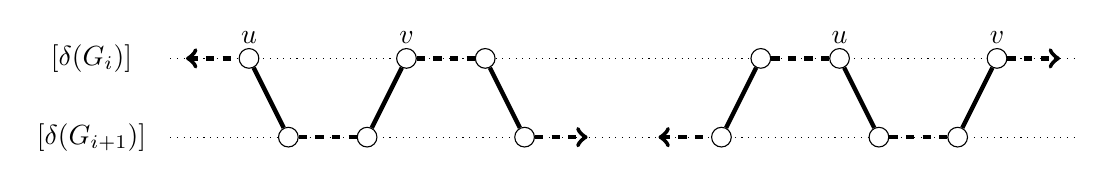
\begin{tikzpicture}[scale=1,auto=left]
  
    \draw[dotted] (0,0) -- (11.5,0);
    \draw[dotted] (0,1) -- (11.5,1);
    
    \node[align=left] at (-1,1) {$[\delta(G_i)]$};
    \node[align=left] at (-1,0) {$[\delta(G_{i+1})]$};
        
    \begin{scope}[every node/.style={circle,draw=black,fill=white,minimum size=0.25cm, inner sep=0}]
    
      \node[label=90:$u$] (u) at (1,1) {};
      \node[label=90:$v$] (v) at (3,1) {};
      \node[] (a) at (1.5,0) {};
      \node[] (b) at (2.5,0) {};
      \node[] (c) at (4,1) {};
      \node[] (d) at (4.5,0) {};
      
      \foreach \from/\to in {u/a,b/v,c/d}
	\draw[ultra thick] (\from) -- (\to);
      
      \foreach \from/\to in {a/b,v/c}
	\draw[dashed,ultra thick] (\from) -- (\to);
	
      \draw[dashed,ultra thick,<-] (0.2,1) -- (u);
      \draw[dashed,ultra thick,->] (d) -- (5.3,0);
      
    \end{scope}
        
    \begin{scope}[shift={(6,0)},every node/.style={circle,draw=black,fill=white,minimum size=0.25cm, inner sep=0}]
    
      \node[] (a) at (1,0) {};
      \node[] (b) at (1.5,1) {};
      \node[label=90:$u$] (u) at (2.5,1) {};
      \node[label=90:$v$] (v) at (4.5,1) {};
      \node[] (c) at (3,0) {};
      \node[] (d) at (4,0) {};
      
      \foreach \from/\to in {a/b,u/c,d/v}
	\draw[ultra thick] (\from) -- (\to);
      
      \foreach \from/\to in {b/u,c/d}
	\draw[dashed,ultra thick] (\from) -- (\to);
	
      \draw[dashed,ultra thick,<-] (0.2,0) -- (a);
      \draw[dashed,ultra thick,->] (v) -- (5.3,1);
      
    \end{scope}
  \end{tikzpicture}
  
  \caption{Repetitive path $P$ composed of vertices of both $B(F)$ and $W(F)$ (in bold). Independently of the start/end layer of the path (left: $[\delta(G_{i+1})]$, right: $[\delta(G_i)]$), it will contain at least three edges between the layers as the colour classes of vertices on both layers are distinct and $P$ is repetitive.}
  \label{fig:three_edges_between_layers}
  
  \end{figure}

By Theorems \ref{thm:facial_outplanar} and \ref{thm:facial_planar_2r}, we get the following corollary:

\begin{corollary}
 Let $G$ be a plane graph. $\pi_f(G) \leq 22$.
 \label{cor:facial_planar}
\end{corollary}

This result improves the previous bound of 24 obtained by Bar{\'a}t and Czap \cite{barat2013facial}.
These bounds of 22 for plane graphs and 11 for outerplane (or 7 if 2-connected) do not seem to be tight. For the Thue number, there exists a plane graph $G$ with $\pi(G) = 11$, and an outerplane graph with $\pi(G)=7$ \cite{barat2007square, dujmovic2012planarlogn}. However, as noted above, there is no known outerplane graph with facial Thue number greater than 4, or plane graph with facial Thue number greater than 5. This suggests the following conjecture:

\begin{conjecture}
 Let $G$ be an outerplane graph. $\pi_f(G) < 11$.
\end{conjecture}

\bibliographystyle{plain}
\bibliography{facial}


% \section*{Appendix: Springer-Author Discount}
% 
% LNCS authors are entitled to a 33.3\% discount off all Springer
% publications. Before placing an order, the author should send an email, 
% giving full details of his or her Springer publication,
% to \url{orders-HD-individuals@springer.com} to obtain a so-called token. This token is a
% number, which must be entered when placing an order via the Internet, in
% order to obtain the discount.

\end{document}
